%!TEX root = ../../thesis.tex
\define{\chapterpath}{\allchapterspath/bci}
\define{\imgpath}{\chapterpath/img}

\chapter{Application to Brain Computer Interaction}
\label{chapter:bci}
\minitoc

We presented an algorithm that exploits task constraints to solve simultaneously a task under human feedback and learn the associated meanings of the feedback signals. We detailed an uncertainty measure than allow our agent to solve this problem more efficiently and shown that our algorithm can transition from task to task in a smooth way. Our algorithm has important practical application since the user can start controlling a device from scratch, without the need of an expert defining the meaning of signals or carrying out a calibration phase. 

In this chapter, we explore the use of our algorithm in brain computer interaction scenario. We consider the grid world reaching task scenario as presented in chapter~\ref{chapter:planning:method}. After briefly presenting the related work, we introduce the experimental setup an the Error-related potential EEG signals we will use. Then, we first test our algorithm with a database of EEG signals and compare the performance of our method with a calibration procedure method (that first collects signal-label pairs during a calibration period and trains a unique classifier). We will highlight one run of our experiments in detail.

% and show  our algorithm conserve good propertie. on EEG signals and has important advantage over calibration based method. 

However, we point out a main difference between calibration procedure and our self-calibration method in that the EEG signals properties can be affected by the action selection of the agent. As our planning method can not guarantee the same agent behavior than during a typical calibration phase, the quality of the signals generated by the users can be impacted. To address this problem, we introduce a prior information of the Error-related potential EEG signals used, namely that the signal corresponding to an ``incorrect'' meaning are more ``powerful'' than the one associated to meaning ``correct''. We will exploit this properties, in addition to our interpretation hypothesis method, and show that we can achieve better performances. 

Finally, we present results where real users teach our artificial agent by assessing agent's actions in their mind, and without calibrating the system beforehand.

The results with real EEG signals allow us to envision that such algorithm could have practical applications in the real word. By removing the need of an expert to collect and calibrate the system, the use of brain computer interfaces may become more practical allowing their users to go out of the labs.

The application of this work to BCI is a collaboration with I{\~n}aki Iturrate and Luis Montesano.

%%%%%%%%%%%%%%%%%%%%%%%%%%%%%%%%%%%%%%%%%%%%%%
%%%%%%%%%%%%%%%%%%%%%%%%%%%%%%%%%%%%%%%%%%%%%%
%%%%%%%%%%%%%%%%%%%%%%%%%%%%%%%%%%%%%%%%%%%%%%
%%%%%%%%%%%%%%%%%%%%%%%%%%%%%%%%%%%%%%%%%%%%%%
%%%%%%%%%%%%%%%%%%%%%%%%%%%%%%%%%%%%%%%%%%%%%%
\section{Learning from error related potentials}
\label{chapter:bci:setupandeeg}

\subsection{The visual naviguation task}

The setup of our online experiment is shown in Figure~\ref{fig:BCIsetup}. Each subject was asked to mentally assess the agent's actions with respect to a given target. The system was not calibrated to decode the user EEG signals beforehand. Once the agent identified a task, and whatever the success or failure of the task identification, the user selected a new goal state randomly, the agent reseted the task likelihoods, propagates the believed labels, and teaching started again. At no point the agent has access to a measure of its performance, it could only refer to the unlabeled feedback signals from the user. There was an action every three seconds. Each experiment lasted 500 actions minimum, after 500 steps we kept running the system until a next task was reached.

\begin{figure}[!htbp]
\centering
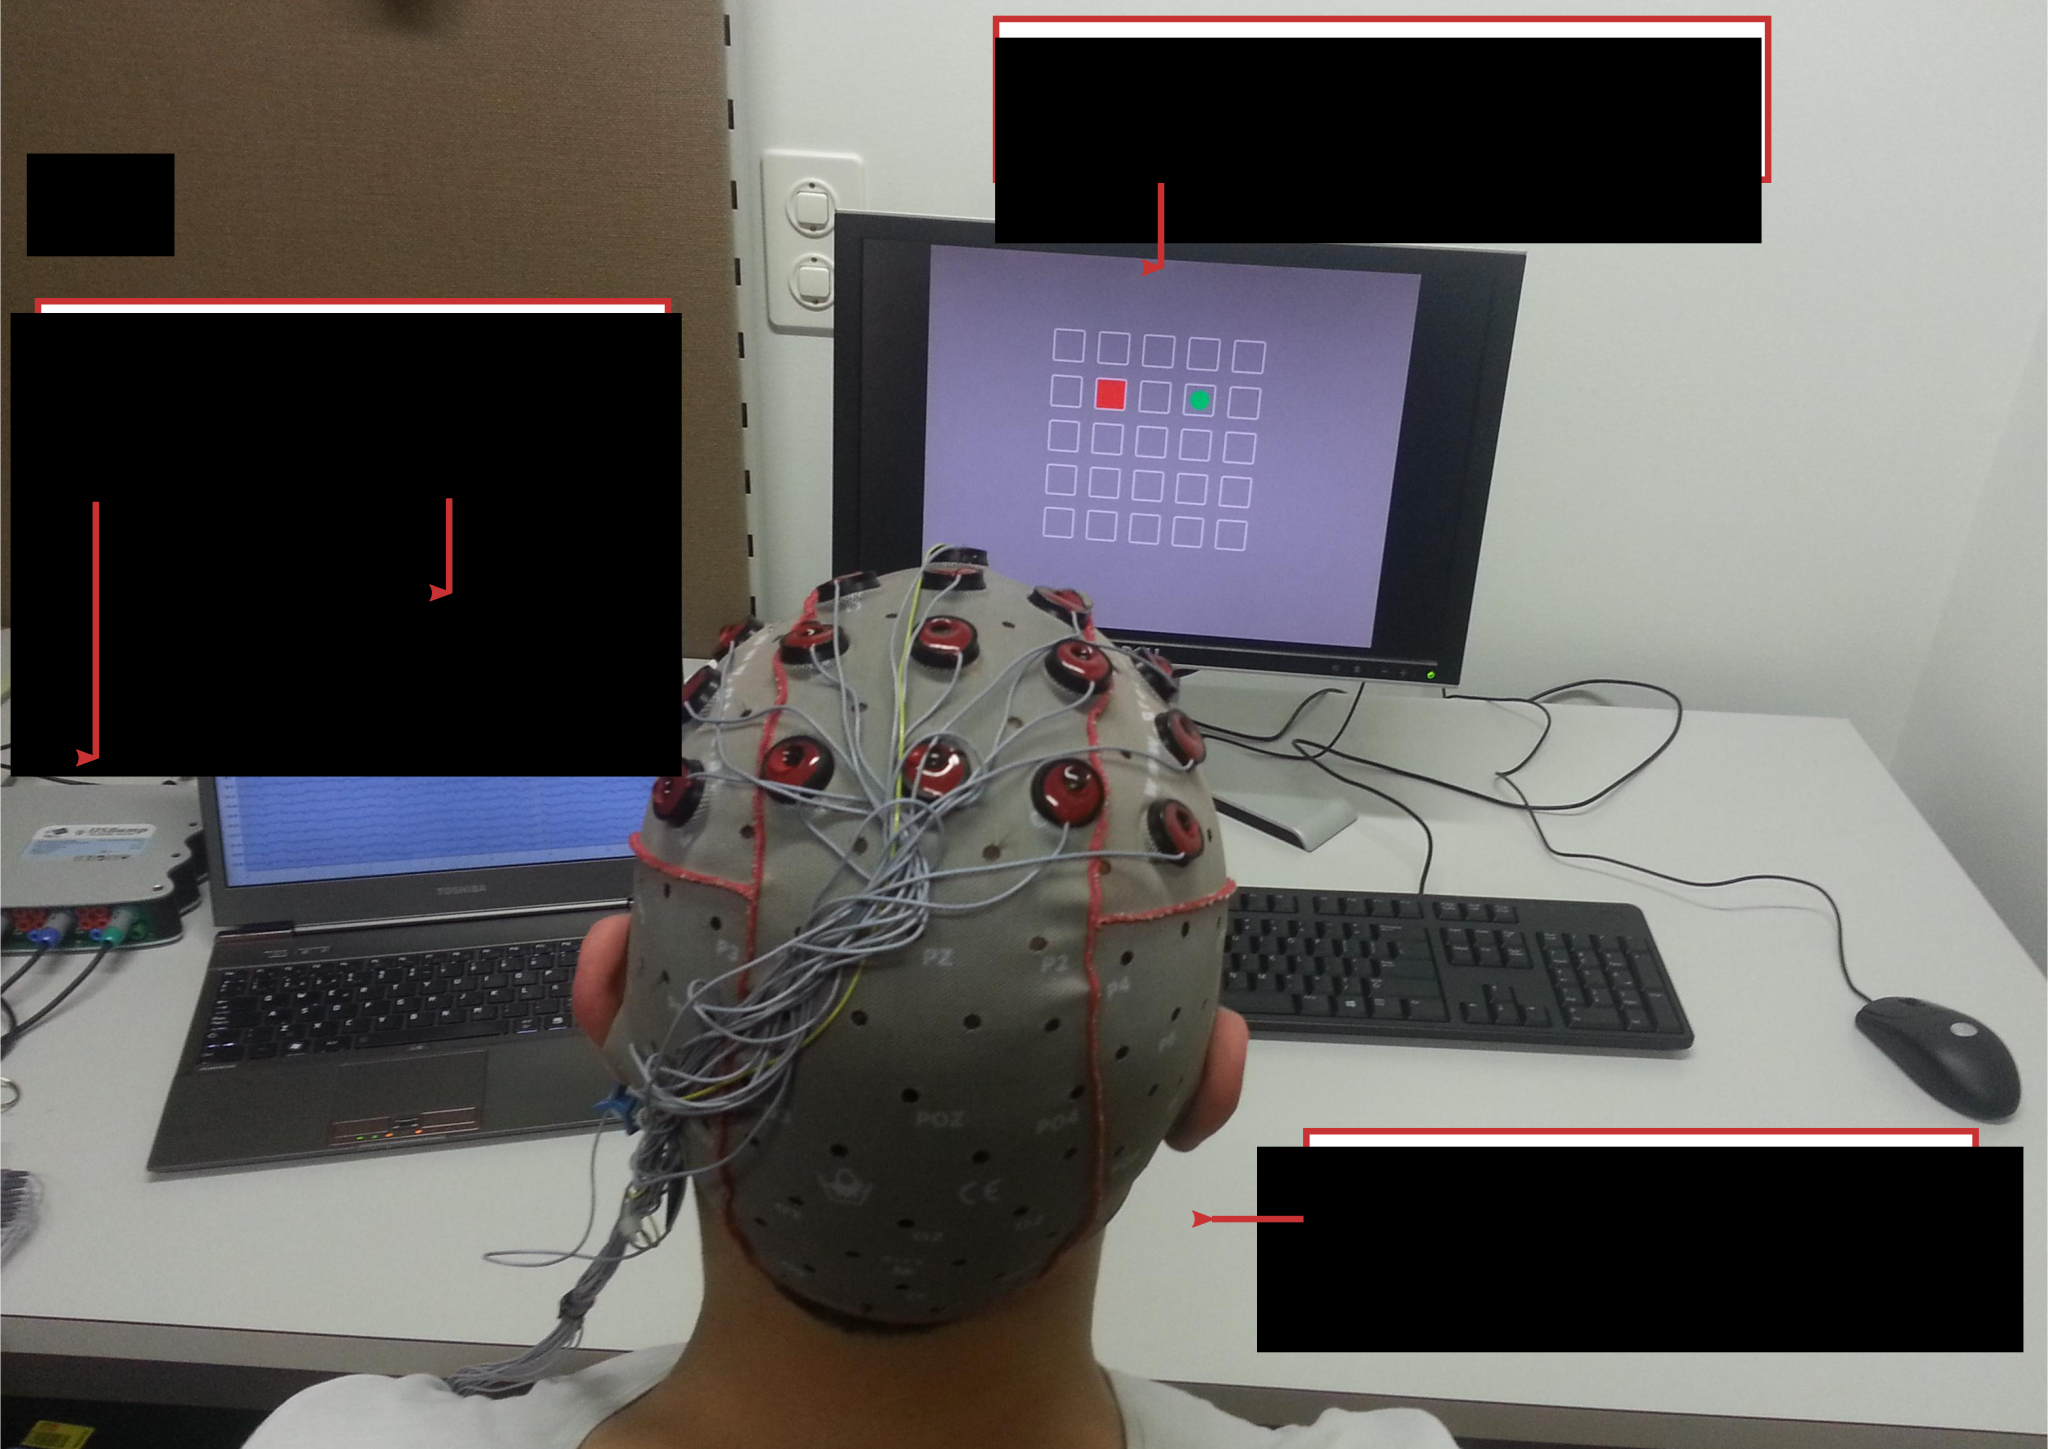
\includegraphics[width=\bcisetupsize\columnwidth]{\visualspdf/onlineXP/setup.pdf}
\caption{The BCI setup for online experiments. On the screen is displayed the grid world with the agent in green. We displayed the intended target in red, which was selected randomly. The purpose of this red square is to help the user remembering the target and our algorithm is at no point aware of the position of this red square.}
\label{fig:BCIsetup}
\end{figure}

\subsection{The brain signals}

As shown in Figure~\ref{fig:EEGsample}, the EEG signals associated to ``incorrect'' labels have slightly more amplitude than the one associated to ``correct'' labels, especially at around 300ms.

\begin{figure}[!htbp]
\centering
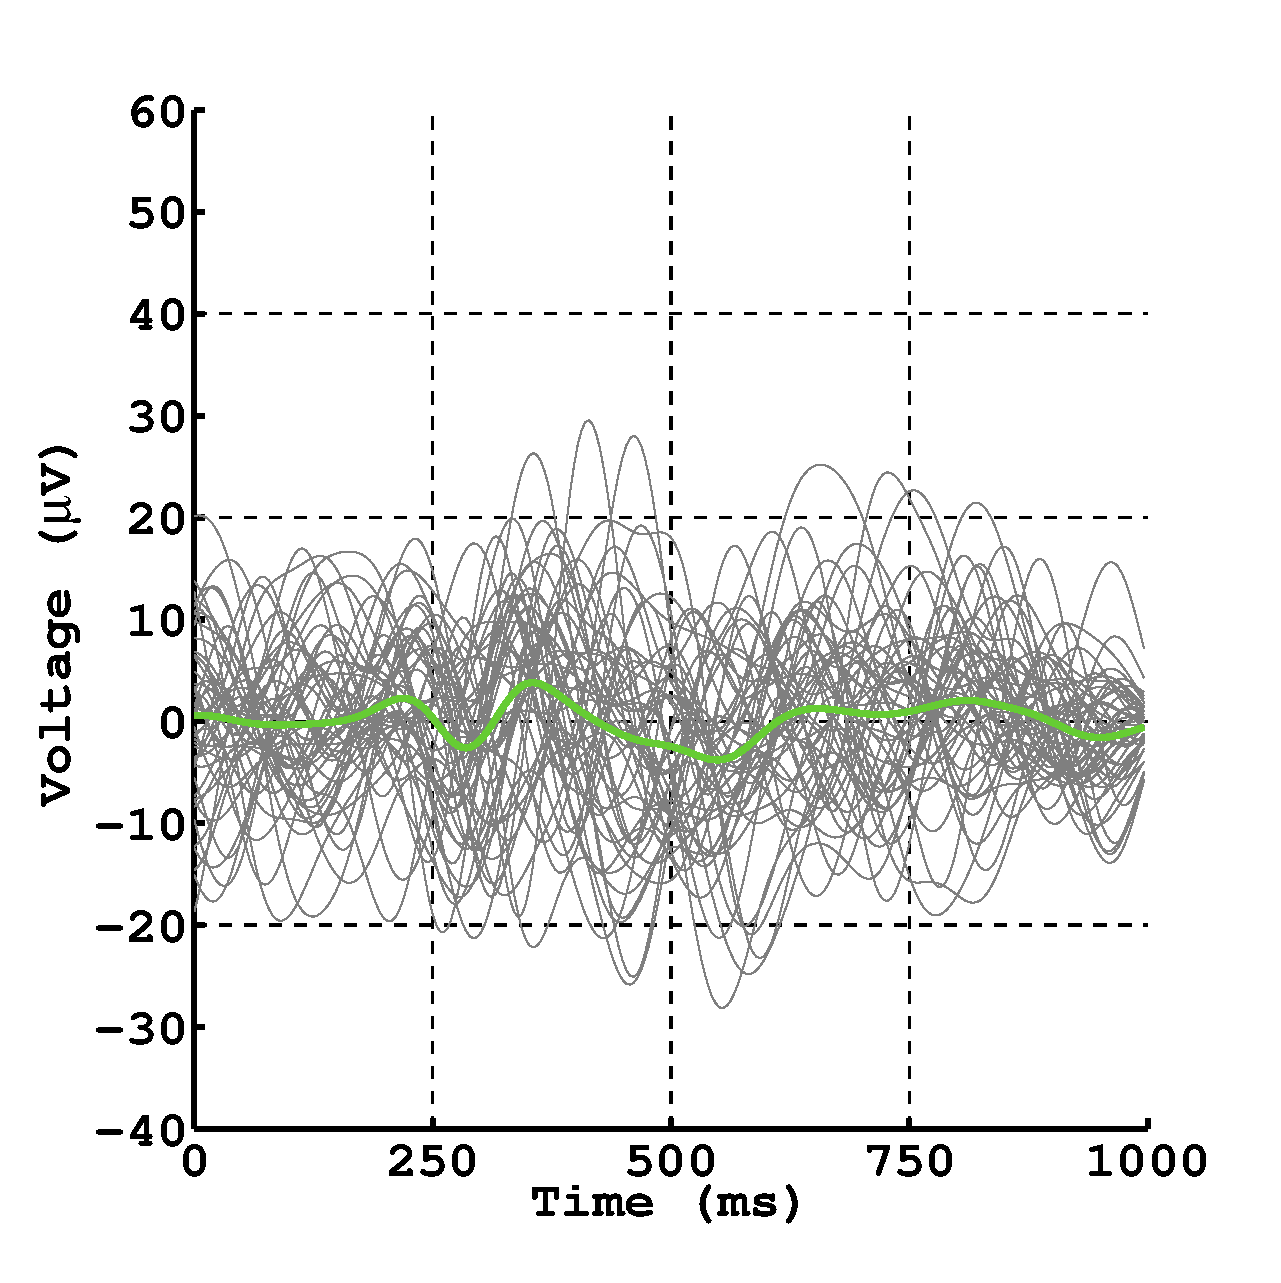
\includegraphics[width=0.49\columnwidth]{\imgpath/illustration/eeg_correct.eps}
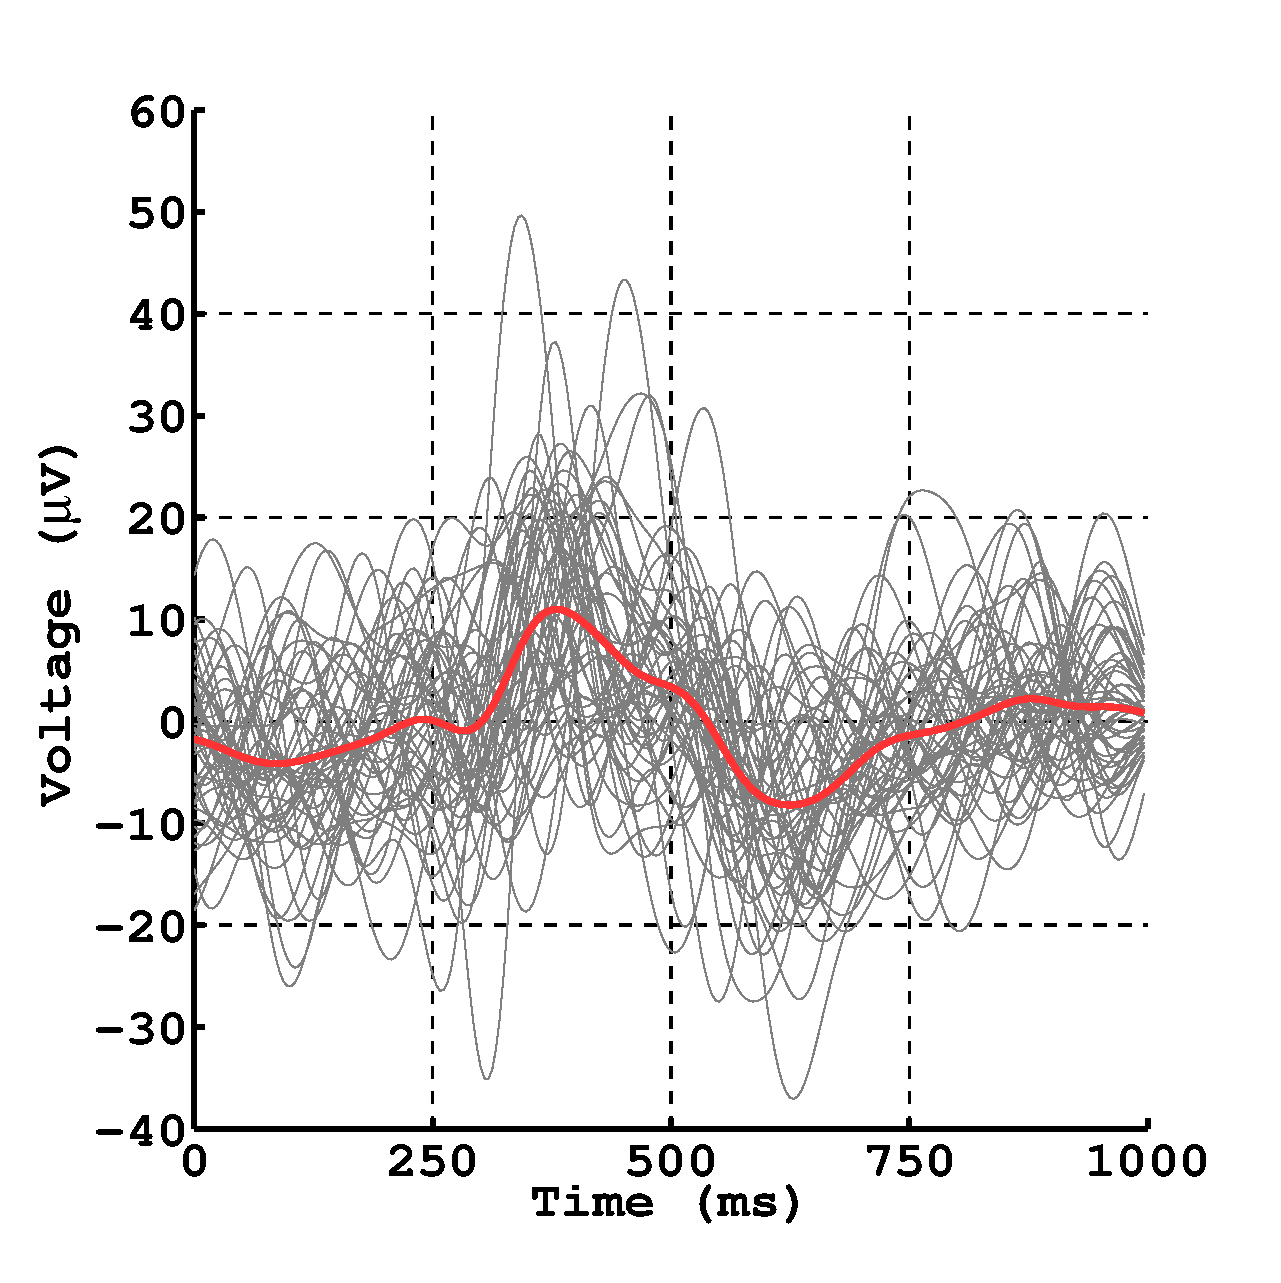
\includegraphics[width=0.49\columnwidth]{\imgpath/illustration/eeg_incorrect.eps}
\caption{Low-pass filtered EEG signals associated to ``correct'' labels (left) and to ``incorrect'' labels (right).  The signals have slightly different amplitudes, especially at around 300ms. \todo{change with one figure inkscaped}}
\label{fig:EEGsample}
\end{figure}

To build our feature vector we consider two fronto-central channels (FCz and Cz) in a time window of $[200,700]$ ms (being 0 ms the action onset of the agent) and downsampled the signal to $32$ Hz. Each element of the feature vector is the value in microvolts of the signal at the corresponding time. To compute the power information contained in our signal we simply compute the sum of the square of each feature representing our signal. This simple approximation allows to capture the slight difference in power between ``incorrect'' and ``correct'' signals (see Figure~\ref{fig:EEGpower}). However this is not enough to classify a single signal with more than 60 percent accuracy, which is almost random. But considering a group of point we can observe that the mean of power of the ``incorrect'' class is higher that the mean power of the ``correct'' class. We will exploit this property as an a priori information of which group of point should means ``correct'' or ``incorrect''.

\subsection{The signal model}

ErrPs signals are generated in the user's brain after s/he assesses actions performed by an external agent \cite{chavarriaga2010learning}, where correct and erroneous assessments will elicit different brain signals. Past approaches have already demonstrated that these signals can be classified online with accuracies of around 80\% and translated into binary feedback, thanks to a prior calibration session that lasts for 30-40 minutes \cite{chavarriaga2010learning, iturrate2013task}.

Following the literature \cite{lotte2007review,blankertz2010single}, we rely on Gaussian classifiers and model the signals using independent multivariate normal distributions for each class, $\mathcal{N}(\mu_c, \Sigma_c), \mathcal{N}(\mu_w, \Sigma_w)$. With $\theta$ the set of parameters $\{\mu_c, \Sigma_c,\mu_w, \Sigma_w\}$. Given the high dimensionality of some datasets we also need to regularize. For this we apply shrinkage to the covariance matrix ($\lambda = 0.5$) and compute the value of the marginal pdf function using a noninformative (Jeffrey's) prior [\cite{gelman2003bayesian}, p88]:

\begin{eqnarray}
p(e|l, \theta) & = & t_{n-d}(e | \mu_l,\frac{\Sigma_l (n+1)}{n(n-d)})
\label{eq:prior}
\end{eqnarray}

where $\theta$ represents the ML estimates (mean $\mu_l$ and covariance $\Sigma_l$ for each class $l$) required to estimate the marginal under the Jeffreys prior, $n$ is the number of signals, and $d$ is the dimensionality of a signal feature vector.

Finally to compute the probability of a label given a signal, we use the bayes rules as follows: 
%
\begin{eqnarray}
    p(l = l_i|e,\theta) &=& \frac{p(e|l = l_i, \theta)p(l = l_i)}{\sum_{k = 1,\ldots, L}{p(e|l = l_k,\theta)p(l = l_k)}}\nonumber \\
    &=& \frac{p(e|l=l_i, \theta)}{\sum_{k = 1,\ldots, L} p(e|l=l_k)} \nonumber
\end{eqnarray}
%
As we do not have a priori knowledge on the user intended meaning, we assume all labels are equiprobables, i.e. $\forall k,~p(l = l_k) = \frac{1}{L}$.

%%%%%%%%%%%%%%%%%%%%%%%%%%%%%%%%%%%%%%%%%%%%%%
%%%%%%%%%%%%%%%%%%%%%%%%%%%%%%%%%%%%%%%%%%%%%%
%%%%%%%%%%%%%%%%%%%%%%%%%%%%%%%%%%%%%%%%%%%%%%
%%%%%%%%%%%%%%%%%%%%%%%%%%%%%%%%%%%%%%%%%%%%%%
%%%%%%%%%%%%%%%%%%%%%%%%%%%%%%%%%%%%%%%%%%%%%%
\section{Using pre-recorded EEG signals}
\label{chapter:bci:EEGsignals}

Before trying out our algorithm with real subject, we test the feasibility of our method using pre-recorded ErrP datasets. The objective of this analysis is to study the scalability of our method to EEG data, which may have different properties than our artificial dataset. We will see that our algorithm maintain good properties with EEG signals.

\subsection{Datasets and scenario}

\paragraph{EEG datasets}  The ErrPs EEG data were recorded in a previous study \cite{iturrate2013task} where participants monitored on a screen the execution of a task where a virtual device had to reach a given goal. The motion of the device could be correct (towards the goal) or erroneous (away from the goal). The subjects were asked to mentally assess the device's movements as erroneous or non-erroneous. The EEG signals were recorded with a gTec system with 32 electrodes distributed according to an extended 10/20 international system with the ground on FPz and the reference on the left earlobe. The ErrP features were extracted from two fronto-central channels (FCz and Cz) within a time window of $[200,700]$ ms (being 0 ms the action onset of the agent) and downsampled to $32$ Hz. This leaded to a vector of $34$ features.

% Note that the scenario used to collect the EEG data was the same as the one we run in our simulated experiment and is the same as the one we will run in our online experiment with real subjects.

\paragraph{Comparison with calibration methods} In order to show the benefit of learning without explicit calibration, we compare our method with a typical supervised BCI calibration procedure. Such calibration procedure requires an experimenter to record enough labeled data from the user. Following the literature on ErrPs \cite{chavarriaga2010learning,iturrate2013task} our training data will consist of 80 percent of positive examples (associated to a correct feedback) and 20 percent of negative examples (associated to an incorrect feedback). ErrPs signals are generated by a user when he observes unexpected agent's behaviors, which explains why, during the calibration phase of their system, researchers uses 80 percent of the time a correct action (i.e. moving towards the goal), and only 20 percent of the time an incorrect action, which is therefore unexpected. Our proposed algorithm is compared with different (but standard) sizes of calibration datasets: 200, 300 and 400 examples.

\subsection{One example detailed}

We use Equation~\ref{eq:matchingfiltercrossvalidation} to compute the likelihood of each task using a 10 fold cross-validation to compute the confusion matrix.

Figure~\ref{fig:sequence} shows one particular run of 500 steps comparing our self-calibration method with a calibration procedure of 400 steps. The two independent runs use a real EEG dataset with $80\%$ ten-fold cross-validation classification accuracy. As our algorithm is operational from the first step, it can estimate the real task when sufficient evidences have been collected. On the other hand, a calibration approach collects signal-label pairs for a fixed number of steps, and use the resulting classifier without updating it. This provokes that, during the calibration phase, no tasks can be learned, substantially delaying the user's online operation. 

Of important interest is the ability of the algorithm to evaluate when sufficient evidence has been collected. The dataset considered is of relatively good quality, and we do not need 400 steps to identify the first task. When doing a calibration procedure, the experiment can not known in advance the quality of each particular subject. Therefore, he must run a calibration for long enough so as to have enough examples to adapt to differences in signals' quality. 

% However, for some subject collecting 100 sample is enough.

\begin{figure}[!htbp]
\centering
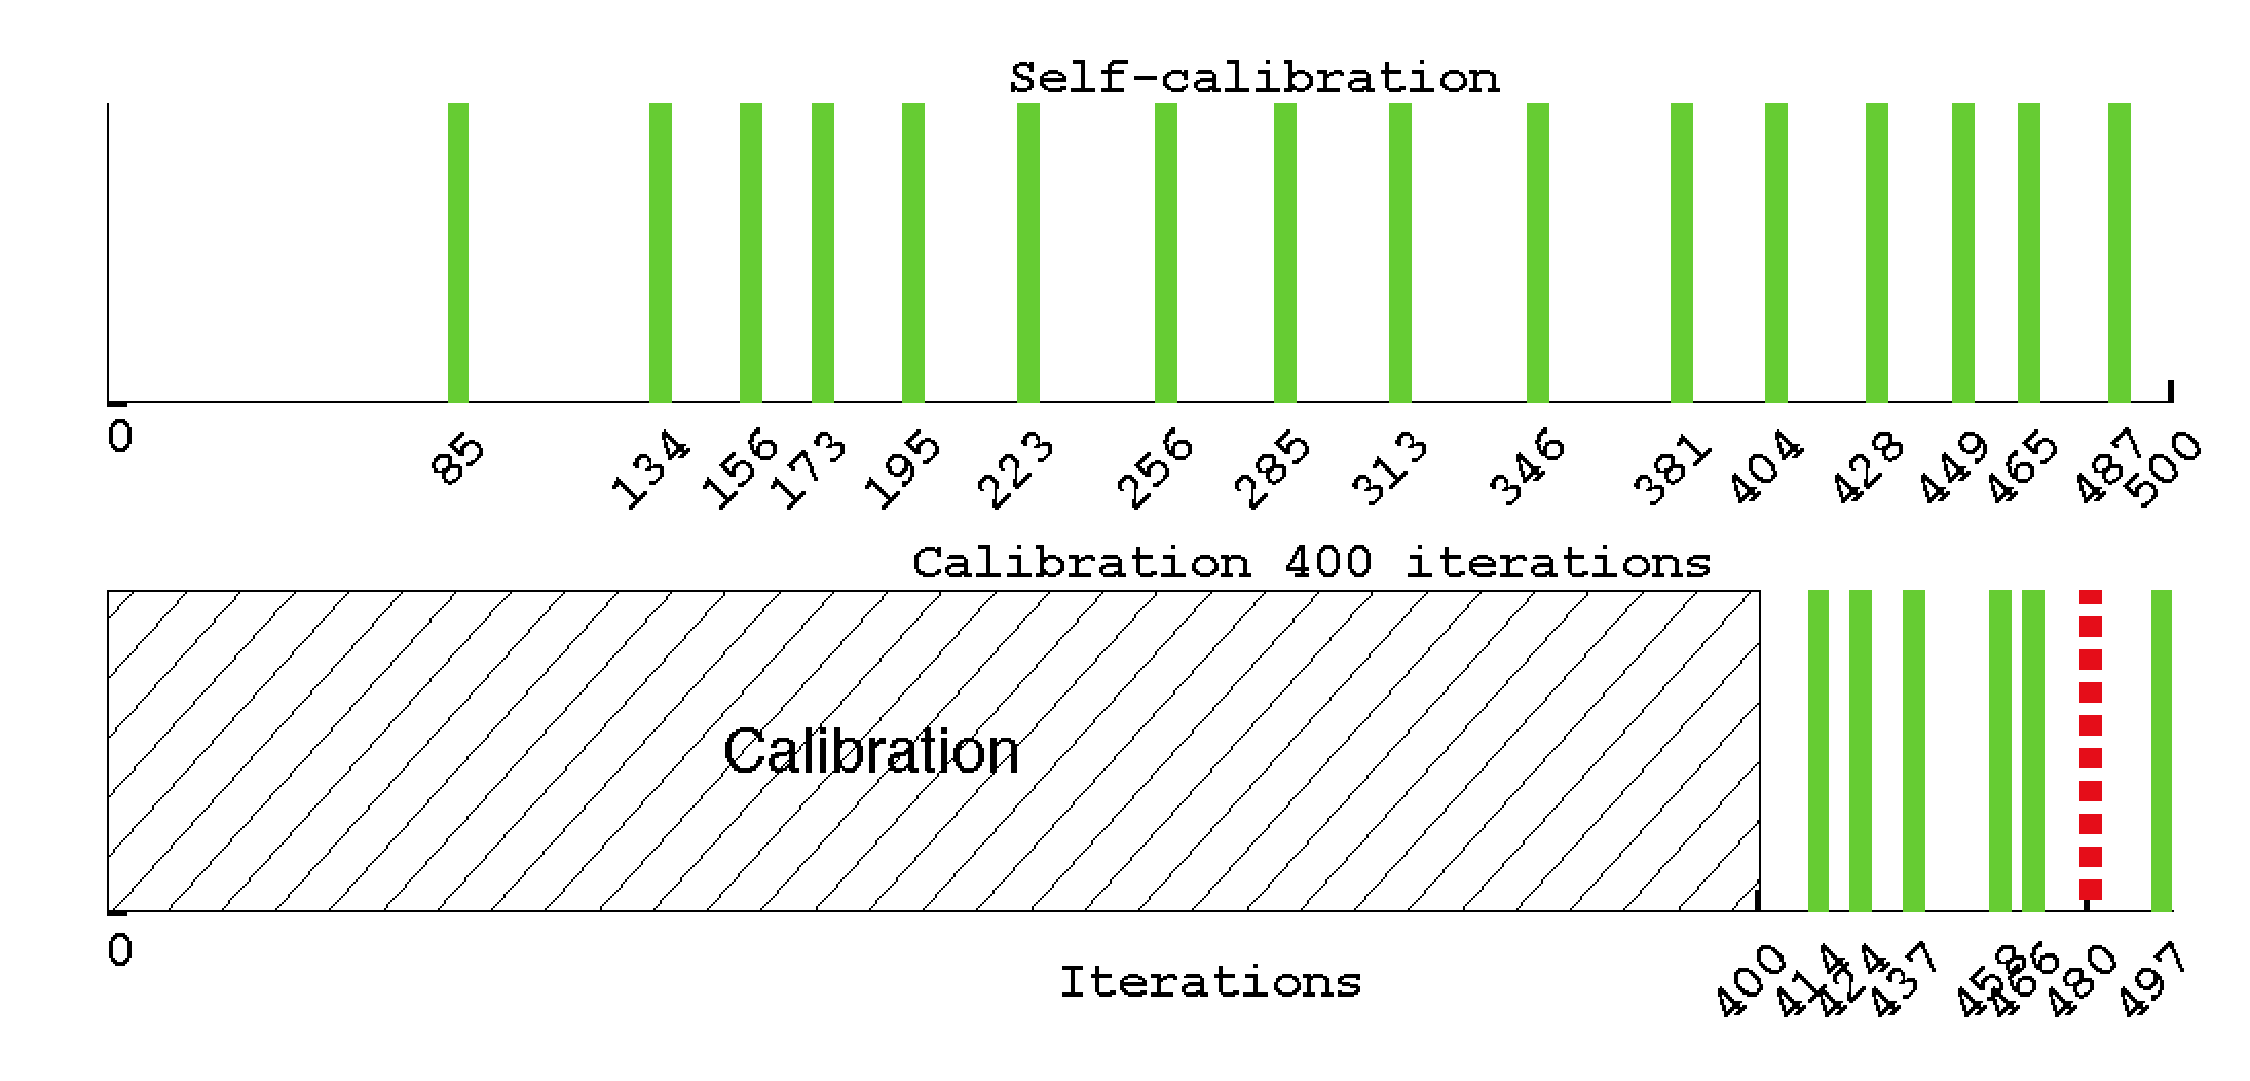
\includegraphics[width=\sequencesize\columnwidth]{\imgpath/plot_the_aaai_sequence.eps}
\caption{Timeline of one run using an EEG dataset of $80$ percent ten-fold cross-validation classification accuracy. Self-calibration (top) versus 400 steps calibration (bottom). Green (filled) and red (dashed) bars represents respectively correct and incorrect task achievements. The proposed self-calibration method allows to reach a first task faster than the it takes to run a calibration procedure.}
\label{fig:sequence}
\end{figure} 

Figure~\ref{fig:sequence_evolution} shows the evolution of classification rate between our self-calibration method and a calibration procedure of 400 steps. As our method assigns different labels to each new teaching signal, the resulting classifiers have different performances, which helps identifying the correct task. Once a task is identified (e.g. step 85 and 134), as explained in chapter~\ref{chapter:lfui:tasttotask}, the corresponding labels are taken as ground truth, and all classifiers will be the same for one iteration. As a consequence, all classifiers have the same accuracies each time a task is competed (e.g. step 85 and 134). As the agent starts exploring again to estimate the new tasks, all the classifiers except the true one will start to have worse accuracies again.

\begin{figure}[!htbp]
\centering
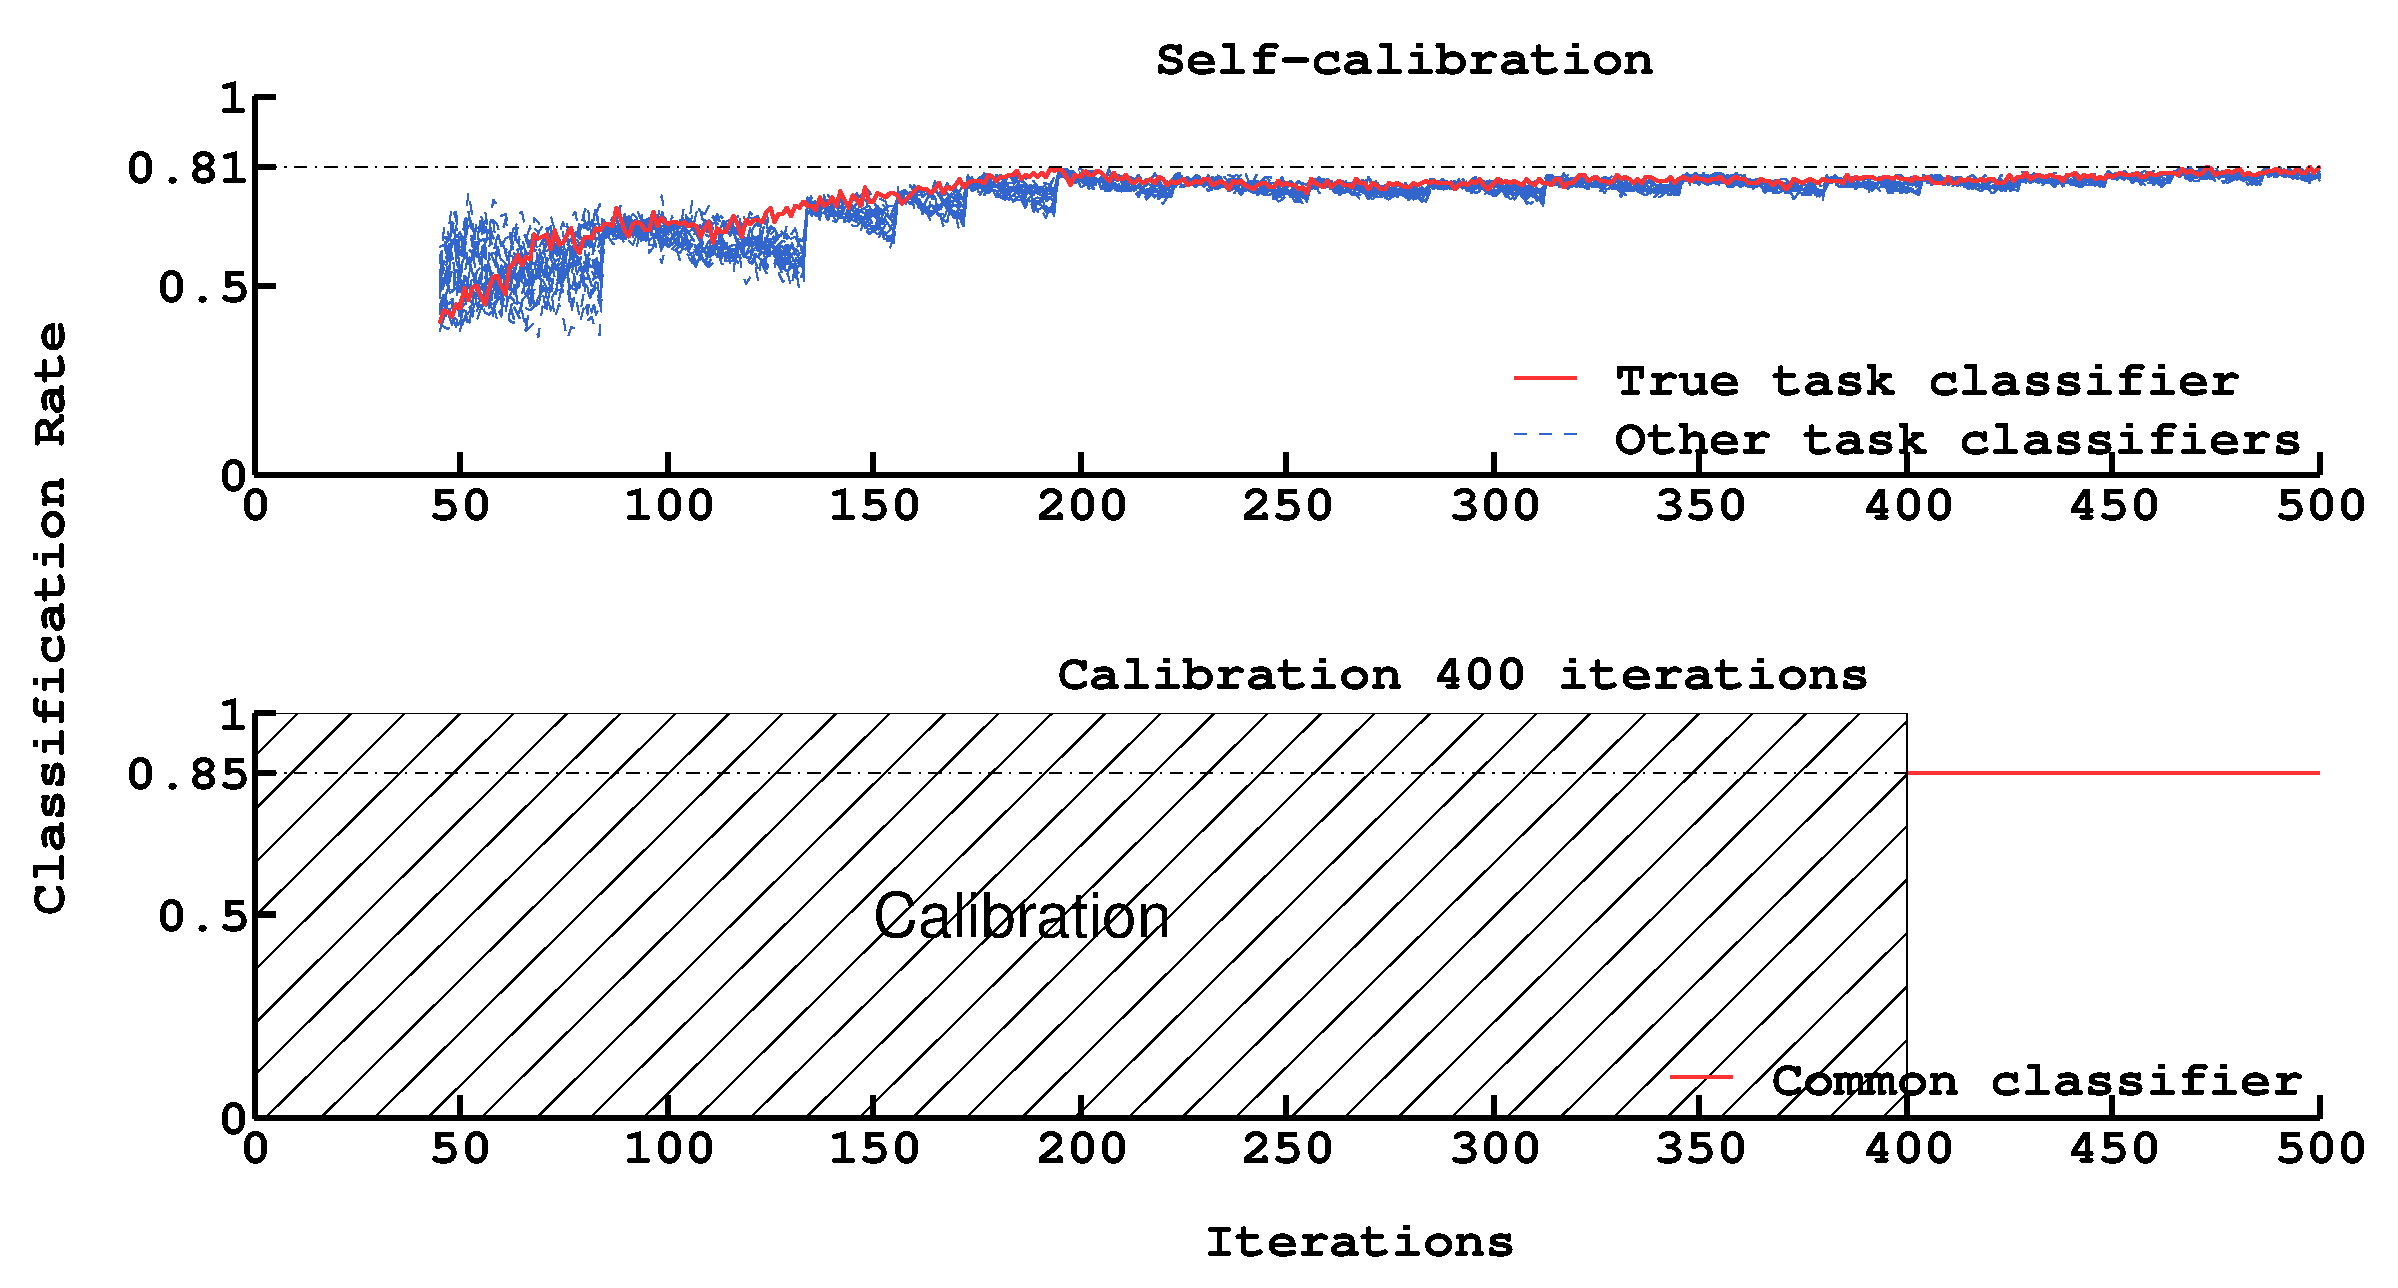
\includegraphics[width=\sequencesize\columnwidth]{\imgpath/plot_evo_classification_rate.eps}
\caption{Evolution of the classification rates of all classifiers for one run using EEG data. Self-calibration (top) versus 400 steps calibration (bottom). On top, the red line represents the classifier corresponding to the successive task taught by the user, the dashed blue lines represent the classifiers of all other tasks. Our method updates 25 classifiers every steps.}
\label{fig:sequence_evolution}
\end{figure}

Before the step 200, we observe a strong evolution of every classifiers (see Figure~\ref{fig:sequence_evolution} top), during this phase the algorithm does not have enough data to create a good classifier of the data and rely mainly on the hypothetic labeling process to differentiate between hypothesis. For example at step 130, the classifier corresponding to the true task is of better quality that all the other one. Therefore, via the estimation of its confusion matrix, its predictions are more trusted than the predictions from the other hypothesis.

However after step 200, the difference between classifier qualities is very small. Indeed, 5 tasks have already been identified and they now share most of their signal-label pairs (due to the propagation of label after each task identified seen in chapter~\ref{chapter:lfui:tasttotask}). From iteration 200, the algorithm behaves similarly if a calibrated classifier common for all hypothesis was provided. Indeed,  all classifier are similar and make similar predictions. 

Interestingly, these two modes are captured by the same equation (see Equation~\ref{eq:matchingcrossvalidation}), which compares predicted and expected labels while taking into account the confidence in the predictions of the classifiers using their respective estimated confusion matrix.

\subsection{Planning}

Figure~\ref{fig:planningEEG} compares the number of steps (with maximum values of 500 steps) needed to identify the first task when learning from scratch with different planning methods. Our proposed planning method guide the agent towards states that maximize disambiguation among hypotheses, which outperforms the other action selection methods. Given these results, the remainder of this section will only consider our planning method.

\begin{figure}[!htbp]
    \centering
    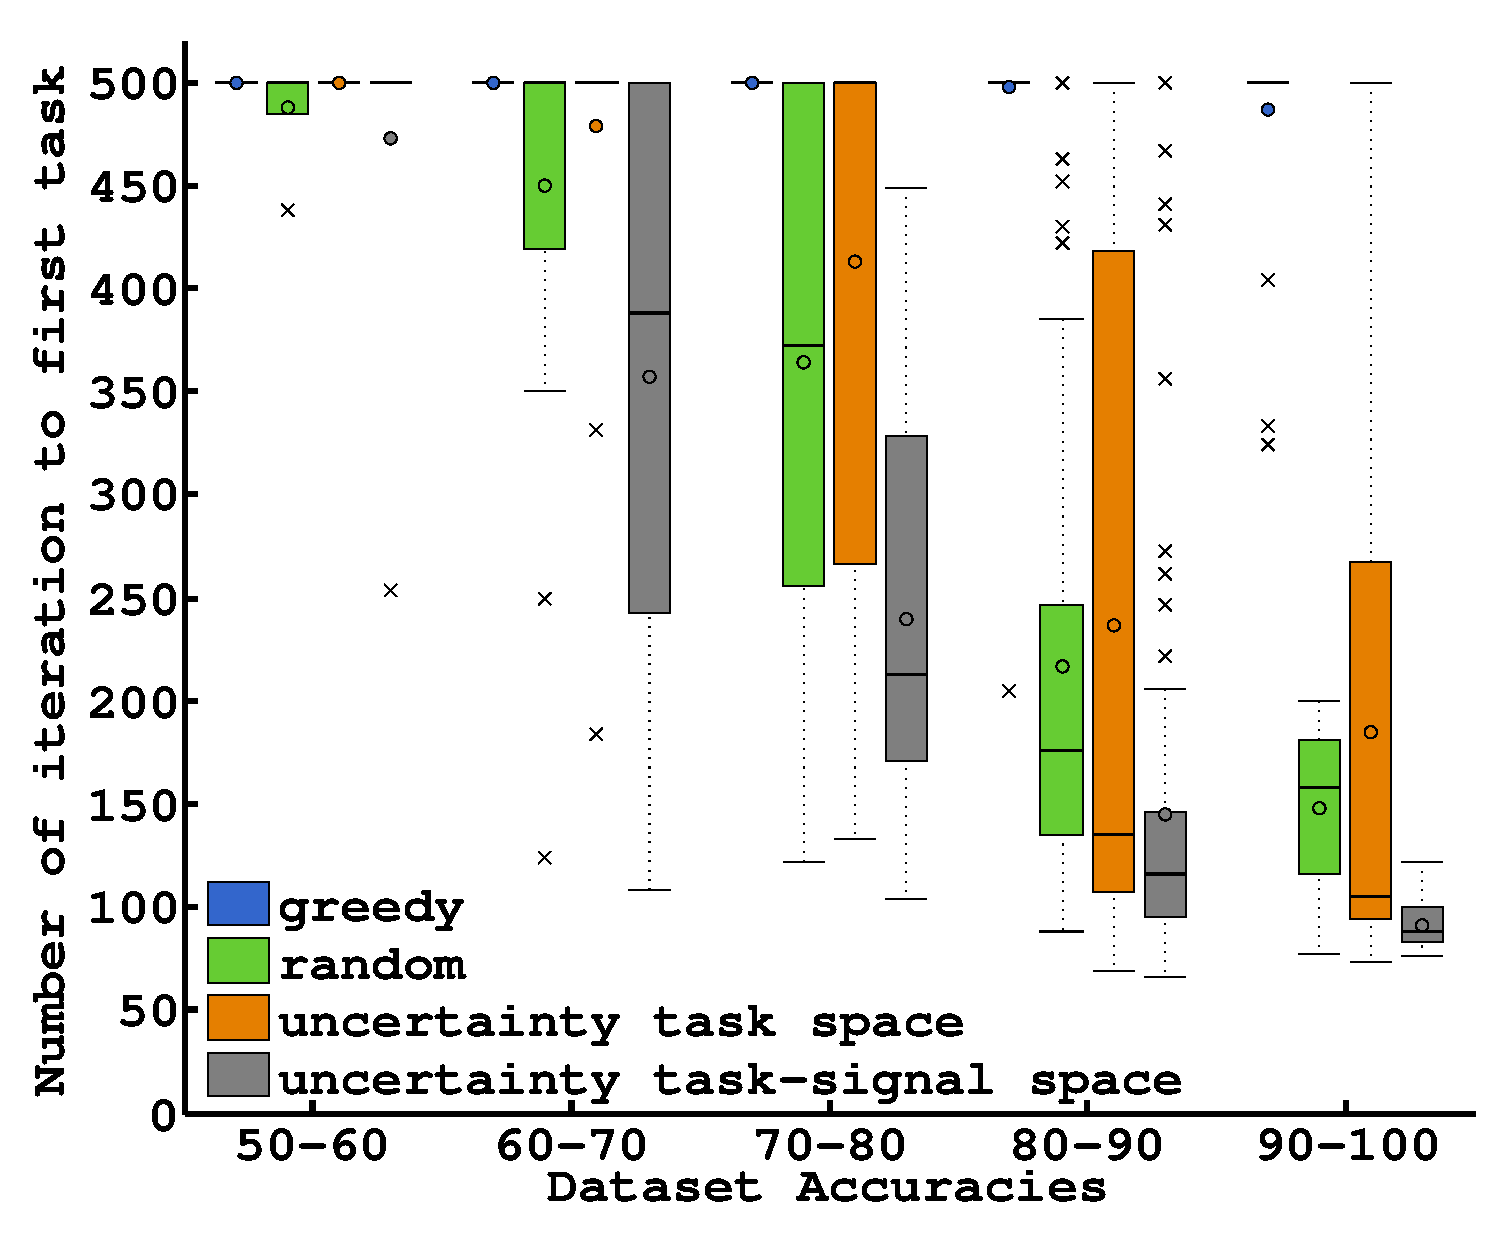
\includegraphics[width=\plotsize\columnwidth]{\imgpath/plot_EEG_planning.eps}
    \caption{Number of steps to complete first task using EEG data of different quality. The EEG data have similar properties than our 30 dimensional simulated data in Figure~\ref{fig:artificialplanning}. Our planning method, based on both the task and the signal to meaning mapping uncertainty, is more efficient that choosing action randomly, greedily, or only based on the uncertainty on the task.}
    \label{fig:planningEEG}
\end{figure}

\subsection{Time to first task}

Figure~\ref{fig:firstEEG} shows the number of iterations needed to identify the first task and compares the results between our self-calibration method and calibration periods of 200, 300, and 400 iterations. The percentage of time the first task was correctly identified is shown on top of each box plot. For our self-calibration method, the learning time is strongly correlated with the dataset quality. This is an important properties, it means our method is able to adapt online to the quality of the data it receives. For datasets of more than 80 percent classification accuracy, we can complete the first task in less than 150 steps on average and without mistake.

\begin{figure}[!htbp]
\centering
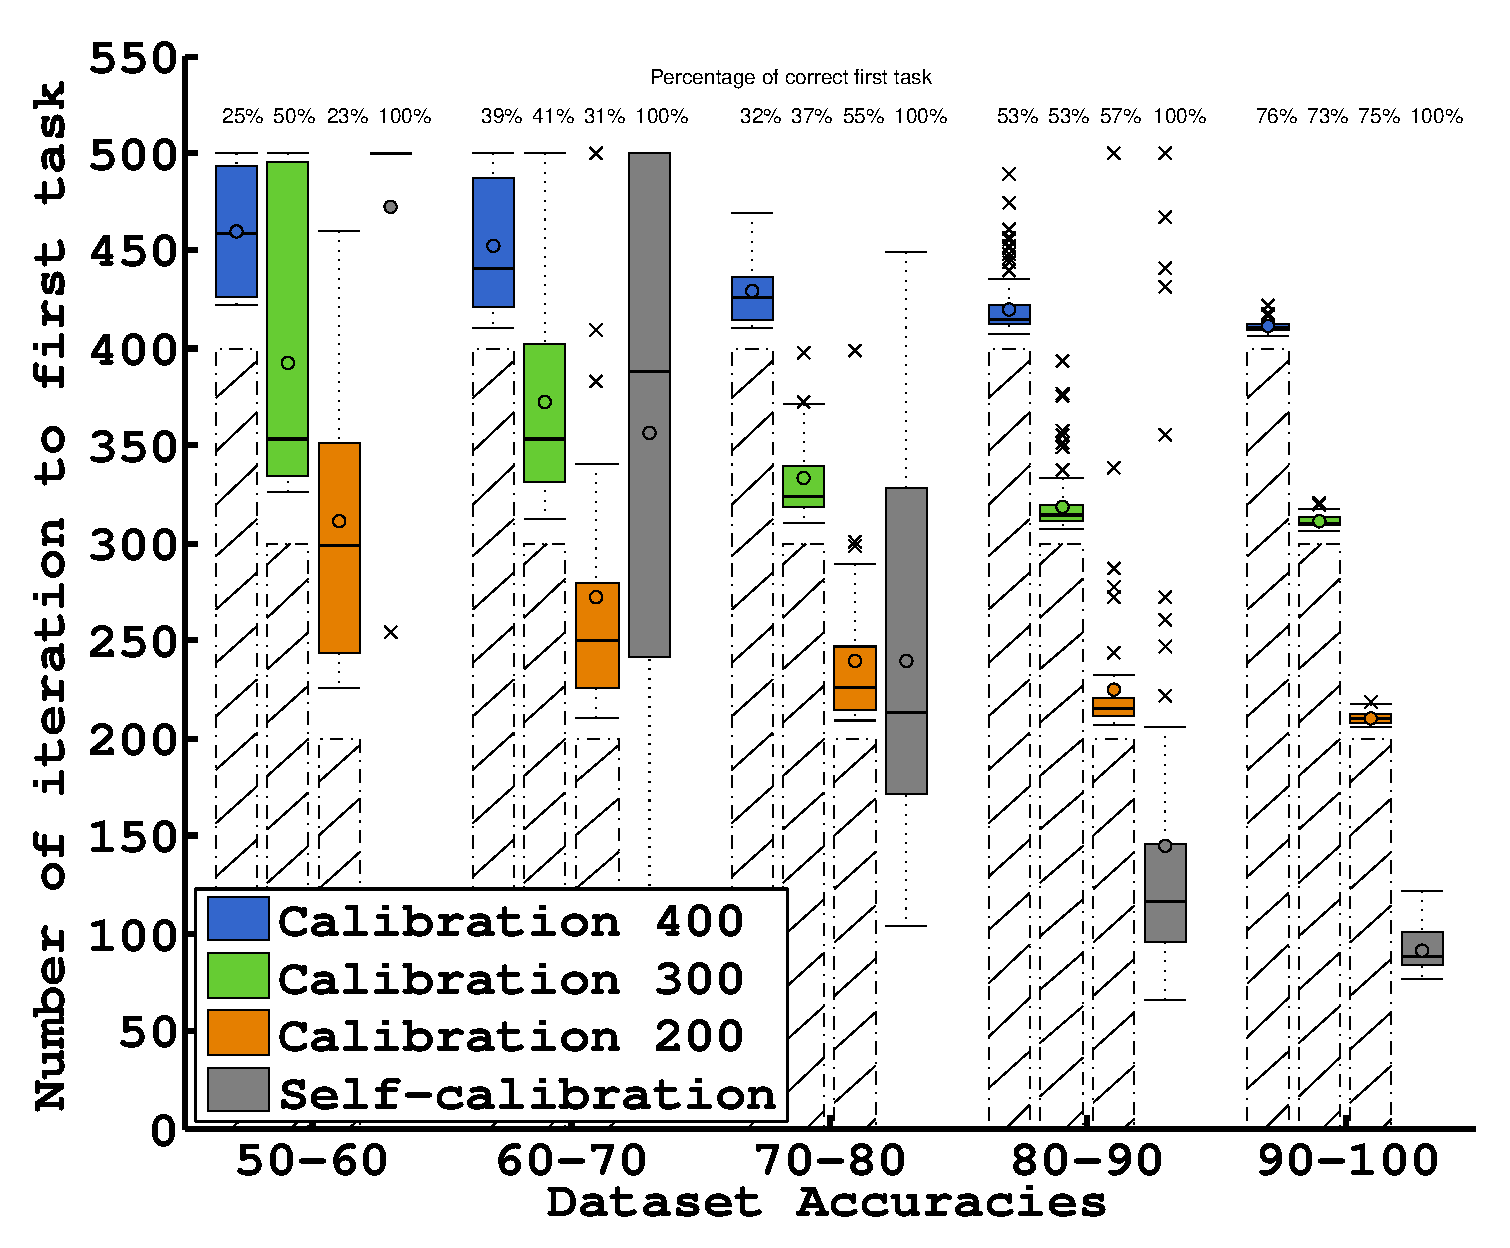
\includegraphics[width=\plotsize\columnwidth]{\imgpath/plot_EEG_calib_firstconf.eps}
\caption{Number of steps to complete the first task using EEG data. The agent plans its action using our uncertainty based method. The percentage of time the first task was correctly identified is shown on top of each box plot. The method scale well to EEG data. For our self-calibration method, the learning time is strongly correlated with the dataset quality. Contrary to the standard calibration approaches, we do not make mistakes with low quality datasets.}
\label{fig:firstEEG}
\end{figure}

Compared to calibration based methods, our algorithm allows to complete the first task without errors. However, calibration based methods, which do not update their classifier once calibrated, identify more tasks incorrectly. In addition, the time to complete the first task is less correlated with the datasets' quality for the calibration based methods than for our self-calibration procedure. Training one classifier per task makes our algorithm more robust. We will discuss propose several explanations of the bad performances of calibration based methods in section~\ref{chapter:bci:cheating}.

\subsection{Cumulative performances}

Figure~\ref{fig:nCorrectEEG} compares the number of tasks achieved in 500 steps. With datasets of more than 90\% classification accuracy, we can achieve more than 20 tasks on average. 

% These results are consistent with artificial dataset analysis.

\begin{figure}[!htbp]
\centering
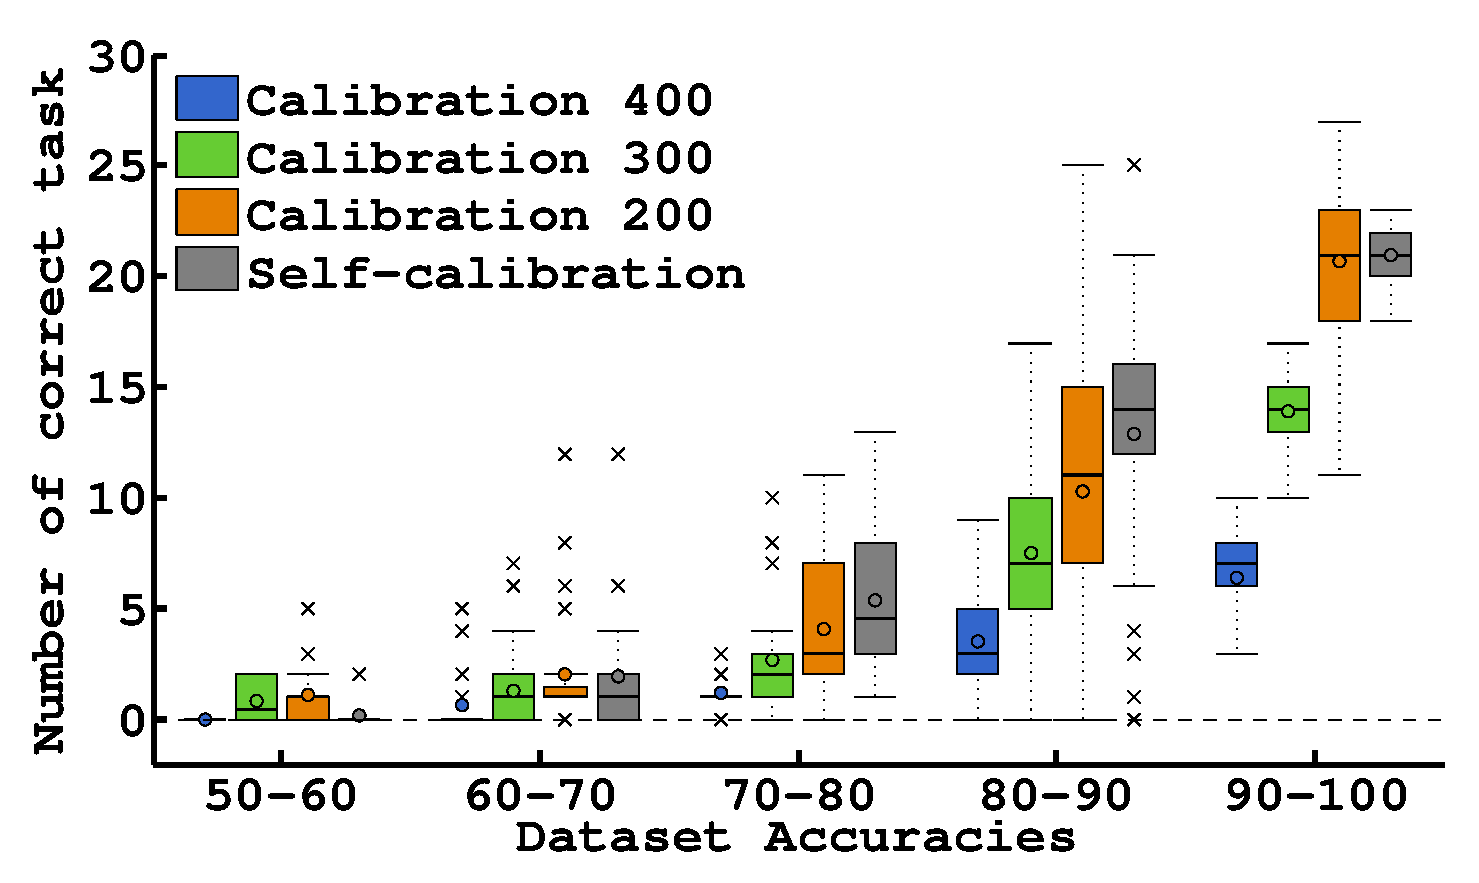
\includegraphics[width=\plotsize\columnwidth]{\imgpath/plot_EEG_calib_nCorrect.eps}
\caption{Number of tasks correctly achieved in 500 steps with EEG data. Calibration based methods can not complete a significant number of tasks because most of the experimental time is spent on calibrating the system.}
\label{fig:nCorrectEEG}
\end{figure} 

The calibration based methods can not complete a significant number of tasks because most of the experimental time is spent on calibrating the system. A calibration of 200 steps allow to reach as many target correctly than the self-calibration method, but it also produces many wrong estimation, see Figure~\ref{fig:nWrongEEG}. For calibration based methods, the less time spent on calibration the poorer the classifier, which implies more mistakes.

\begin{figure}[!htbp]
\centering
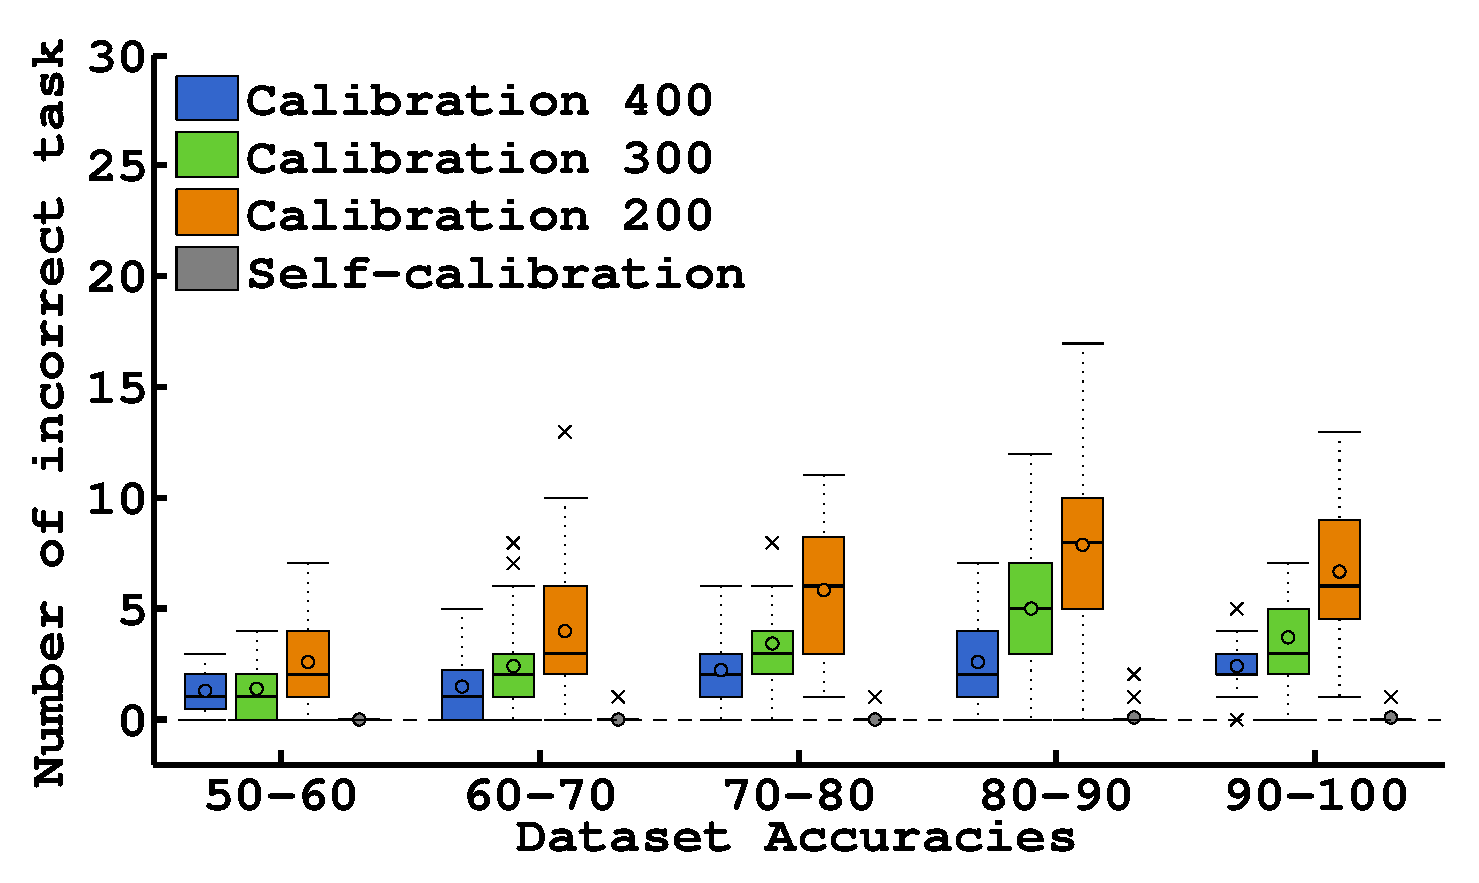
\includegraphics[width=\plotsize\columnwidth]{\imgpath/plot_EEG_calib_nWrong.eps}
\caption{Number of tasks incorrectly achieved in 500 steps with EEG data. Calibration based methods, which do not update their models once calibrated, make more errors.}
\label{fig:nWrongEEG}
\end{figure}

\subsection{Last 100 iterations performances}

Figure~\ref{fig:nCorrectEEG_last100} compares the number of tasks achieved during the last 100 steps with EEG data. During the last 100 steps, all methods are active at their full potential because no time is lost in calibrating the system. With dataset in the range of 80-90\%, all methods achieve an average success rate of one task every 20 steps. However calibration based methods, which do not update their classifiers once calibrated, make more mistakes (see figure \ref{fig:nWrongEEG_last100}). While our method achieve slightly less task during the last 100 steps, it makes less mistakes, which seems to indicate our method is more conservative. We will discuss that point in section~\ref{chapter:bci:cheating}.

\begin{figure}[!htbp]
\centering
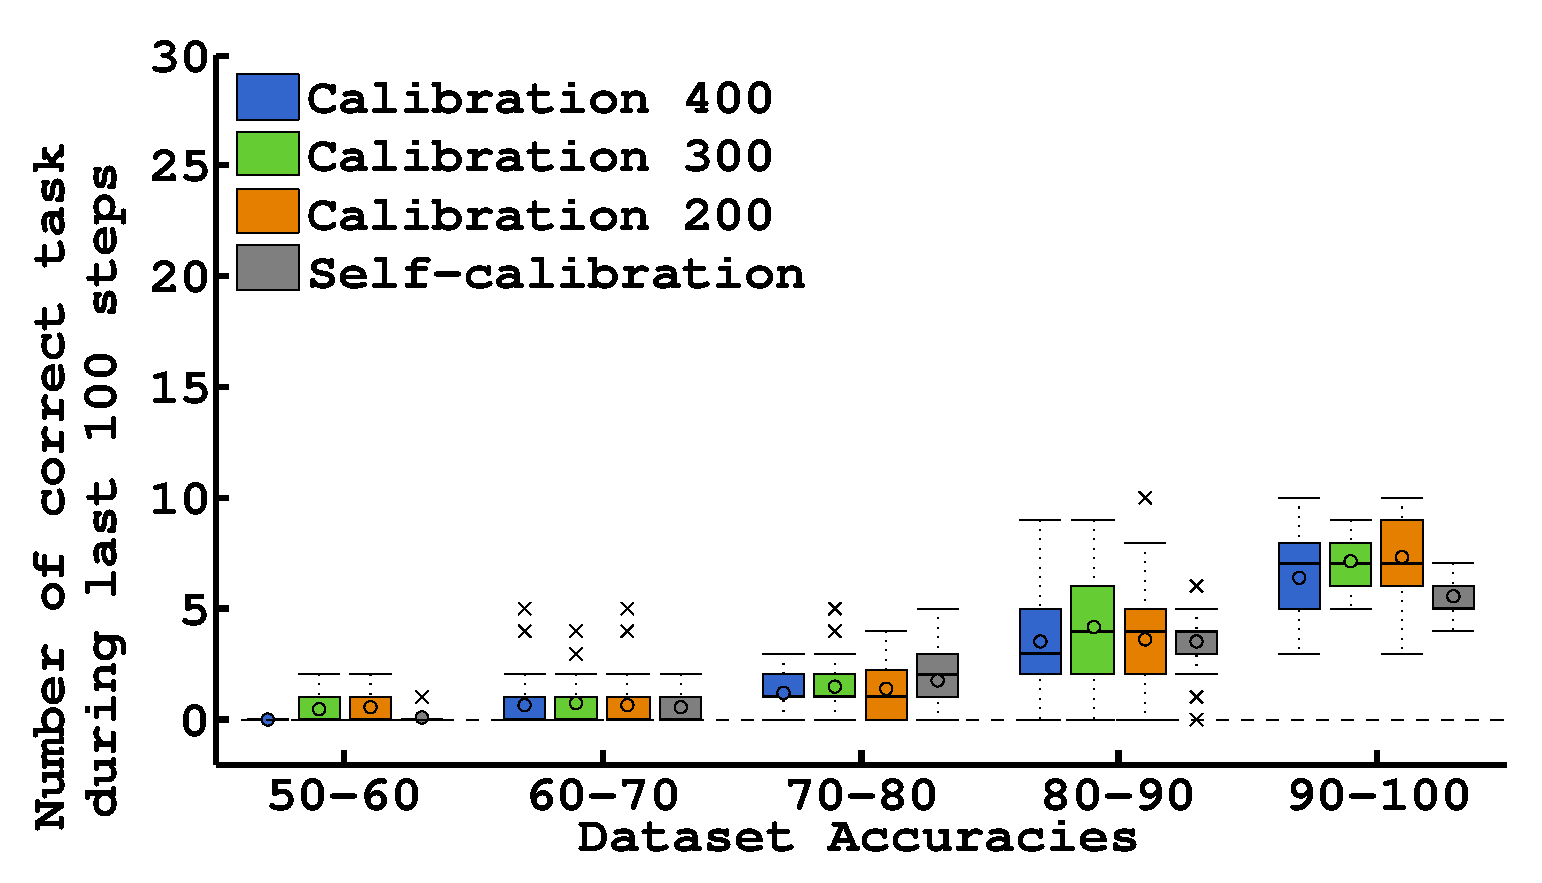
\includegraphics[width=\plotsize\columnwidth]{\imgpath/plot_EEG_calib_nCorrect_last100.eps}
\caption{Number of tasks correctly achieved during the last 100 steps using EEG data. All methods allow the agent to complete an equivalent of tasks.}
\label{fig:nCorrectEEG_last100}
\end{figure} 

\begin{figure}[!htbp]
\centering
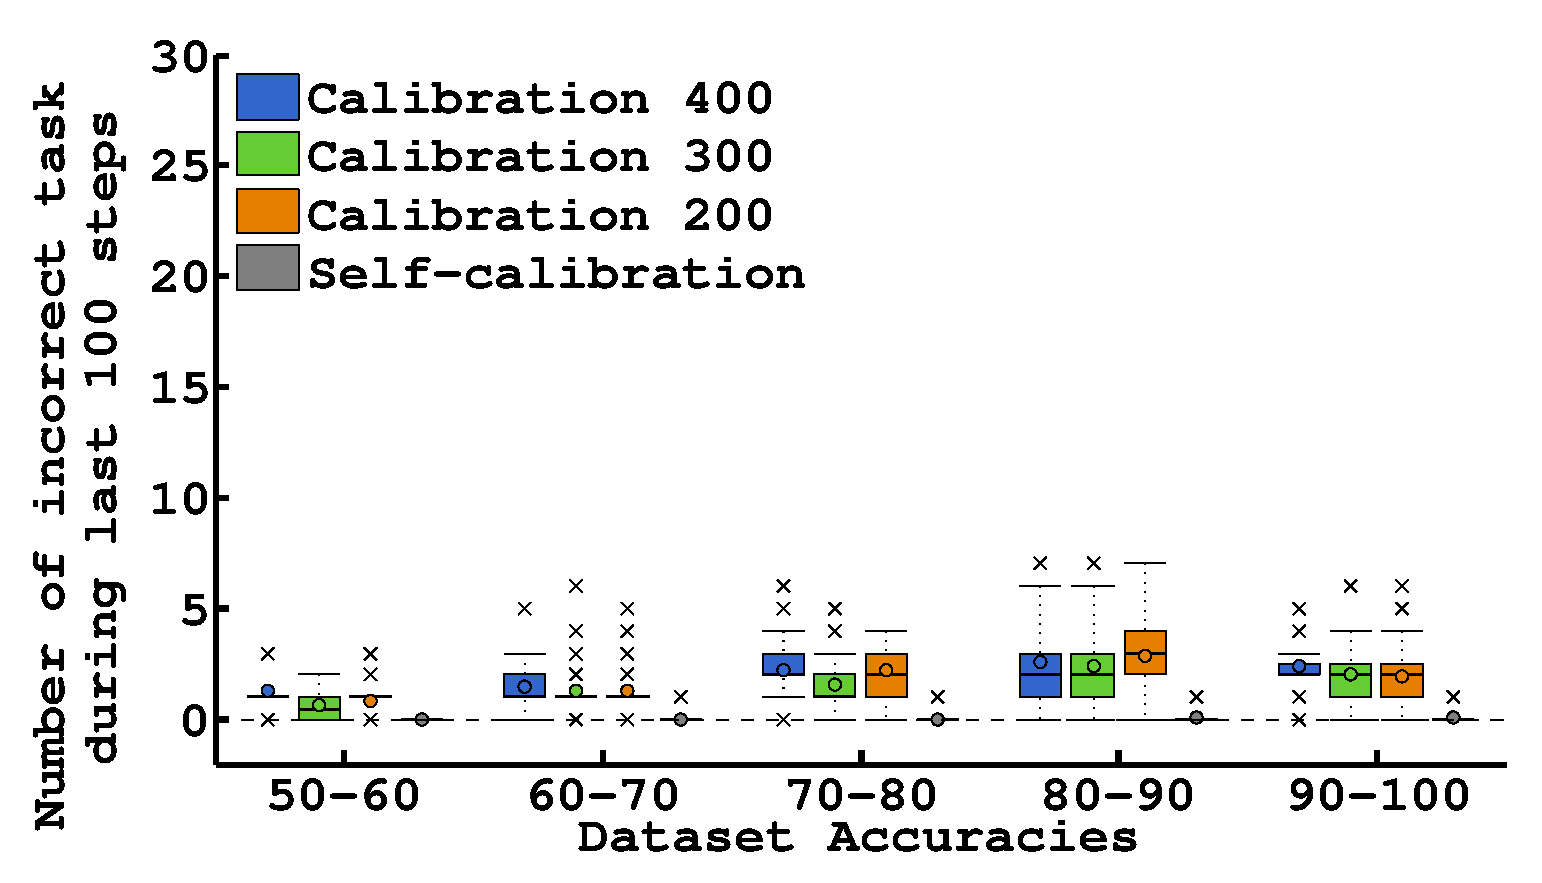
\includegraphics[width=\plotsize\columnwidth]{\imgpath/plot_EEG_calib_nWrong_last100.eps}
\caption{Number of tasks incorrectly achieved during the last 100 steps using EEG data. Calibration based methods, which do not update their classifiers once calibrated, make more errors.}
\label{fig:nWrongEEG_last100}
\end{figure} 

%%%%%%%%%%%%%%%%%%%%%%%%%%%%%%%%%%%%%%%%%%%%%%
%%%%%%%%%%%%%%%%%%%%%%%%%%%%%%%%%%%%%%%%%%%%%%
%%%%%%%%%%%%%%%%%%%%%%%%%%%%%%%%%%%%%%%%%%%%%%
%%%%%%%%%%%%%%%%%%%%%%%%%%%%%%%%%%%%%%%%%%%%%%
%%%%%%%%%%%%%%%%%%%%%%%%%%%%%%%%%%%%%%%%%%%%%%
\section{Why are we cheating with pre-recorder EEG samples?}
\label{chapter:bci:cheating}

For this BCI scenario, we can identify two main differences between our self-calibration method and the usual calibration based approaches:
\begin{enumerate}
\item \textbf{Online update of multiple classifiers.} Our method integrates new data at each new step, and classifiers can differ between task hypothesis. For incorrect task hypothesis, the signal-label pair added to the training datasets can be incorrect and decrease the performance of the associated classifier. This dynamic can be observed in figure \ref{fig:sequence_evolution}, where classifiers associated to incorrect tasks (in blue) have lower estimated accuracy than the classifiers associated to the correct task (in red). As a result, our algorithm makes different predictions and updates for each hypothesis.
\item \textbf{Positive/Negative percent ratio of training examples}. Following the literature \cite{chavarriaga2010learning, iturrate2013task}, the training dataset for calibration based methods was composed of 80 percent of the signals of meaning ``correct'', and only 20 percent of ``incorrect''. The ratio obtained during the self-calibration experiments is more balanced (around 50/50, see Table~\ref{tab:correctLabelRatio}), resulting in classifiers with better properties. But, during online real world experiments, a 50/50 percent ratio may lead to practical problems and should be studied in more details.
\end{enumerate}

This latter aspect concerning the positive/negative ratio of training example is usually required due to the properties of the signal we seek for in the subjects' brain. Indeed ErrP signals are more powerful when triggered by non expected movement of the agent, rather than being a voluntary erroneous assessment. In other words, for the ErrP signal to be observable and of good intensity, the user should not expect the agent to make a mistake. This explains why, during the calibration phase of their system, researchers uses 80 percent of the time a correct action (i.e. moving towards the goal), and only 20 percent of the time an incorrect action which is therefore unexpected \cite{chavarriaga2014errare}. This is possible during a calibration period because both the experiment informs both the user the agent of the task to consider. As the agent knows the task, it can plan its action to maintain a 80/20 percent meaning ratio.

However, i our learning scenario, the agent is not aware of the task the user has in mind. Therefore it is impossible to guarantee a 80/20 percent ratio of positive/negative examples. In practice, using our approach, the agent acquires as many signals of meaning ``correct'' than of meaning ``incorrect'' according to the true intended task, see Table~\ref{tab:correctLabelRatio}.

\begin{table}
\centering
\rowcolors{2}{gray!25}{white}
\begin{tabular}{c c c}
Dataset Accuracies & Self-calibration & Calibration \\ \hline
50-60 & 0.48 (0.02) & 0.8 (0) \\
60-70 & 0.50 (0.03) & 0.8 (0) \\
70-80 & 0.53 (0.03) & 0.8 (0) \\
80-90 & 0.57 (0.03) & 0.8 (0) \\
90-100 & 0.59 (0.01) & 0.8 (0) \\
\end{tabular}
\caption{Mean ratio of positive examples in the training datasets (standard deviation shown in parenthesis). Calibration procedures for creating a usable dataset of ErrP signals usually account for a 80 percent ratio of positive examples. However, when the task is unknown, it is impossible to guarantee such ratio. In practice, using our self-calibration method, an agent will collect as many positive than negative examples. This is likely to impact the quality of the ErrP signals received from the human brain during online experiments.}
\label{tab:correctLabelRatio}
\end{table}

At a glance, our observation of the ratio of positive/negative signals can explain the results of Figure~\ref{fig:firstEEG}, Figure~\ref{fig:nWrongEEG}, and Figure~\ref{fig:nWrongEEG_last100}, where the calibration based methods, while using the same update equation, make more mistakes than our self-calibration method. Apart from the fact that our method train one classifier per class, calibrating using 400 examples should produce similar results than our self-calibration approach. But after 400 steps, the calibration based method only observed 80 signals corresponding to the ``incorrect'' class, while the self-calibration method observed 200 signals. As the signals are represented in a 34 dimensional space, 80 samples may not be enough to build a good model, especially for low quality datasets.

% As a results, the properties of the classifiers are different between our self-calibration method and the one from the calibration procedure.

Figure~\ref{fig:calibFail} shows the difference between the perceived accuracy of the classifiers (i.e. when estimating their quality on their training data) versus the actual accuracy of the classifiers (i.e. when estimating their quality on the remaining data in our bigger dataset). For dataset of good quality, our method generates classifiers that are under-confident while the calibration method tend to produce over-confident classifiers. This over-confidence is likely to explain the higher number of estimation errors when relying on a calibration procedure, versus the very low error rate observed with our self-calibration method which tend to under-estimate the quality of its classifiers.

\begin{figure}[!htbp]
\centering
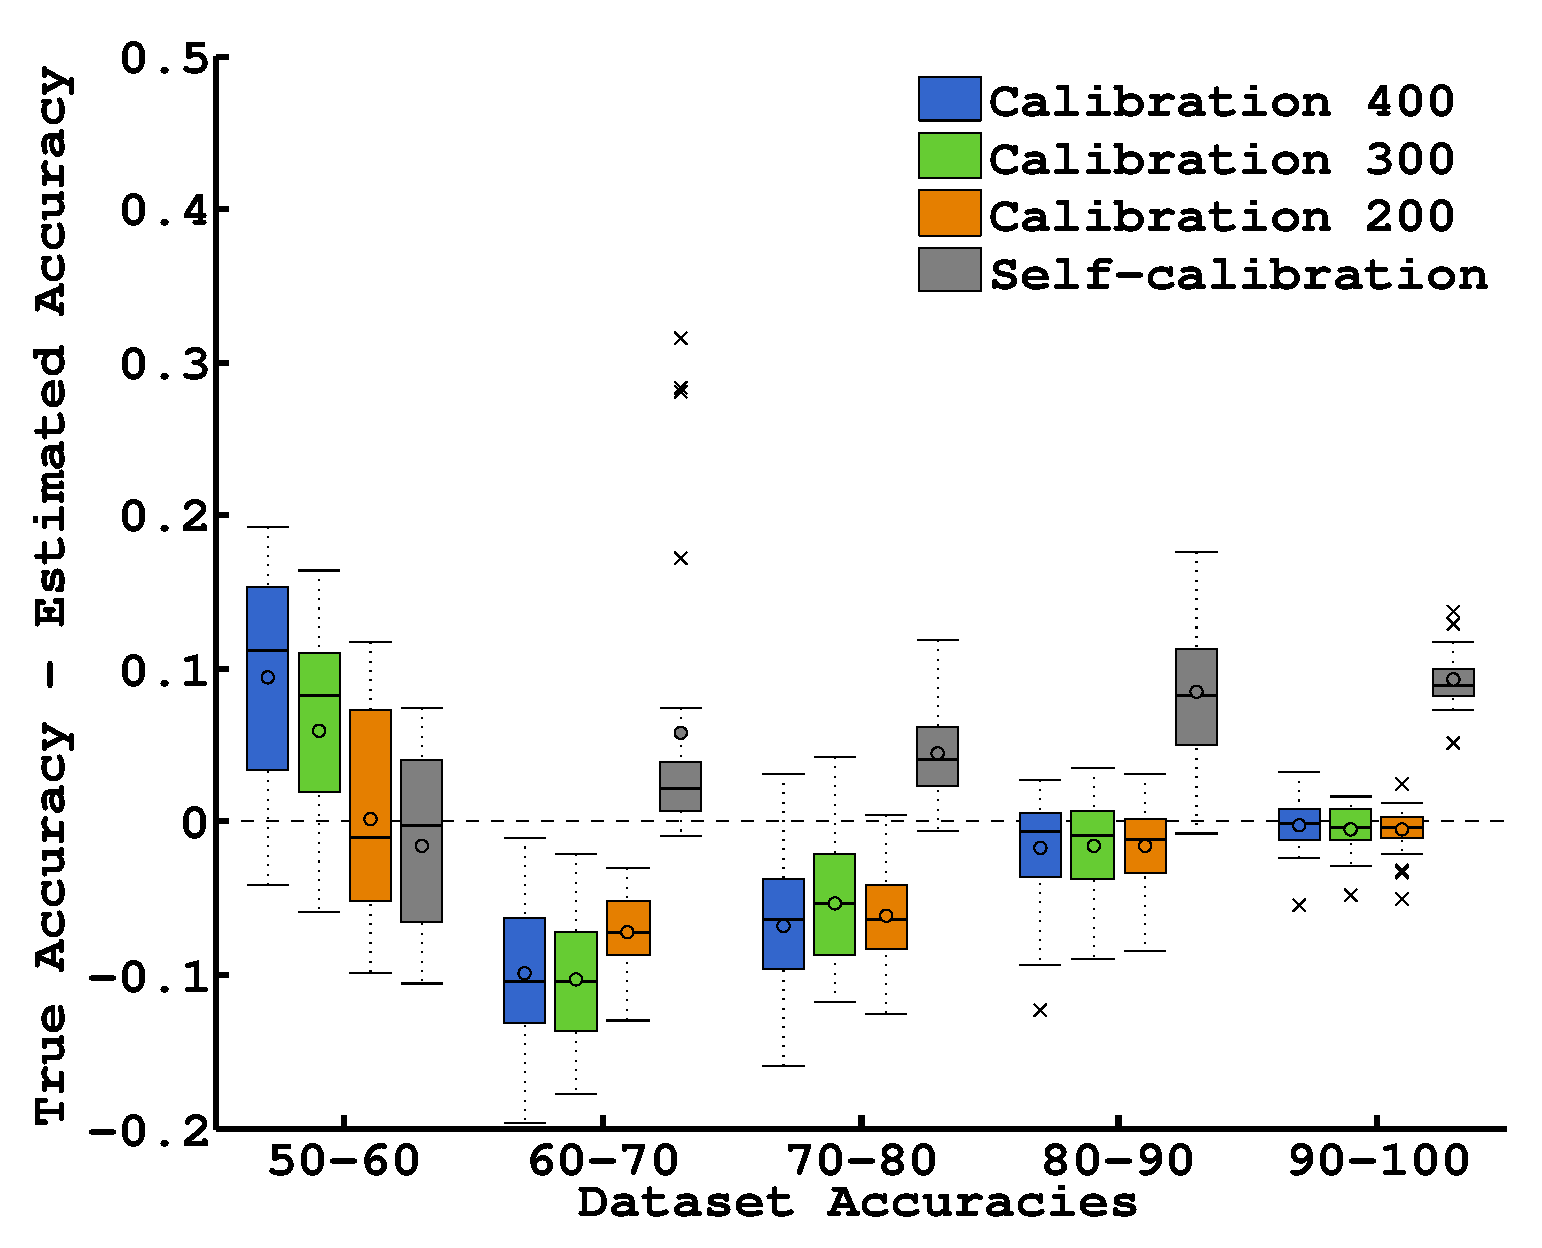
\includegraphics[width=\plotsize\columnwidth]{\imgpath/plot_explaination_for_calib_failure.eps}
\caption{Difference between ``true accuracy'' and estimated accuracy. ``True accuracy'' is the performance of the classifier on the unused data. Estimated accuracy is the 10 fold cross validation performance of the classifier on the training data. A negative(positive) value indicates the classifier is over(under)-estimating its performance. Calibration methods tend to produce over-confident classifiers, certainly due to the biased positive to negative training example ratio, see table \ref{tab:correctLabelRatio}.}
\label{fig:calibFail}
\end{figure}

While this conclusion seems satisfying and is likely to explain the observation made in the previous section, we remind here that the data used in our simulated experiments were collected using an 80/20 percent ratio between the correct and incorrect signal samples. Will the brain signals conserve similar properties when using our self-calibration method online? This is unlikely due to the 50/50 percent ratio of signals' meaning observed using our method. 

The work of Chavarriaga et al. and Iturrate et al. shows that high variability in the teaching signals properties are observed when varying the task and the teaching protocol \cite{chavarriaga2010learning, iturrate2013task}. Indeed ErrP signals are elicited more from non expected movements of the agent than they are voluntary erroneous assessment. In other words, for the ErrP signal to be observable and of good intensity, the user should not expect the agent to make a mistake. With a 50/50 percent ratio, the subject is unlikely to be surprise and may produce signal of lower quality.

During our first experiment with real subject, we observed that the quality of the received data were very poor, even for subjects that were highly trained to the brain assessment task. The main cause was that the behavior of the agent was very confusing with respect to the goal state. The agent seems to act randomly, without trying to move toward the target. Therefore subjects had a lot of difficulty to generated ErrP signals of good quality, which makes the process longer, do not improve the behavior of the agent and further reduces the engagement of the users in the teaching task. Studying in more details the impact of the agent behavior on the ErrP signals is not an objective of this thesis. We acknowledge that a thorough analysis is required to provide more firm conclusion.

Consequently, while some subjects succeeded in the teaching task, we observed a relatively high number of errors and long teaching time. Therefore, in order to improve the learning time and the behavior of the agent, we decided to include an a priori information in the system. This information relates to the difference in power (sum of the EEG feature squared) between EEG signals of meaning ``correct'' and ``incorrect''. The signals related to the unexpected, erroneous action, are, on average, more powerful. But this property alone is not enough to identify ``correct'' and ``incorrect'' signals. In next section, we study in more detail the power component of ErrP signals and present how it can be exploited in our system.

%%%%%%%%%%%%%%%%%%%%%%%%%%%%%%%%%%%%%%%%%%%%%%
%%%%%%%%%%%%%%%%%%%%%%%%%%%%%%%%%%%%%%%%%%%%%%
%%%%%%%%%%%%%%%%%%%%%%%%%%%%%%%%%%%%%%%%%%%%%%
%%%%%%%%%%%%%%%%%%%%%%%%%%%%%%%%%%%%%%%%%%%%%%
%%%%%%%%%%%%%%%%%%%%%%%%%%%%%%%%%%%%%%%%%%%%%%
\section{Including Prior Information}
\label{chapter:bci:priorpower}

In this section, we detail how we can exploit the difference of power between positive and negative ErrP signals. Positive ErrP signals are slightly more powerful that negative ErrPs. Hence, the measuring the power of a signal provide an absolute information about the meaning of a given signal. While this property is not enough to classify with good accuracy ``correct'' and ``incorrect'' signals, we will see that it allows to differentiate between symmetric hypothesis, which improves the performances of our algorithm as well as the perceived behavior of the agent at run time.

\subsection{Difference of power between correct and incorrect signals}

As shown in Figure~\ref{fig:EEGsample}, the EEG signals associated to ``incorrect'' labels have slightly more amplitude than the one associated to ``correct'' labels, especially around 300ms. 

\begin{figure}[!htbp]
\centering
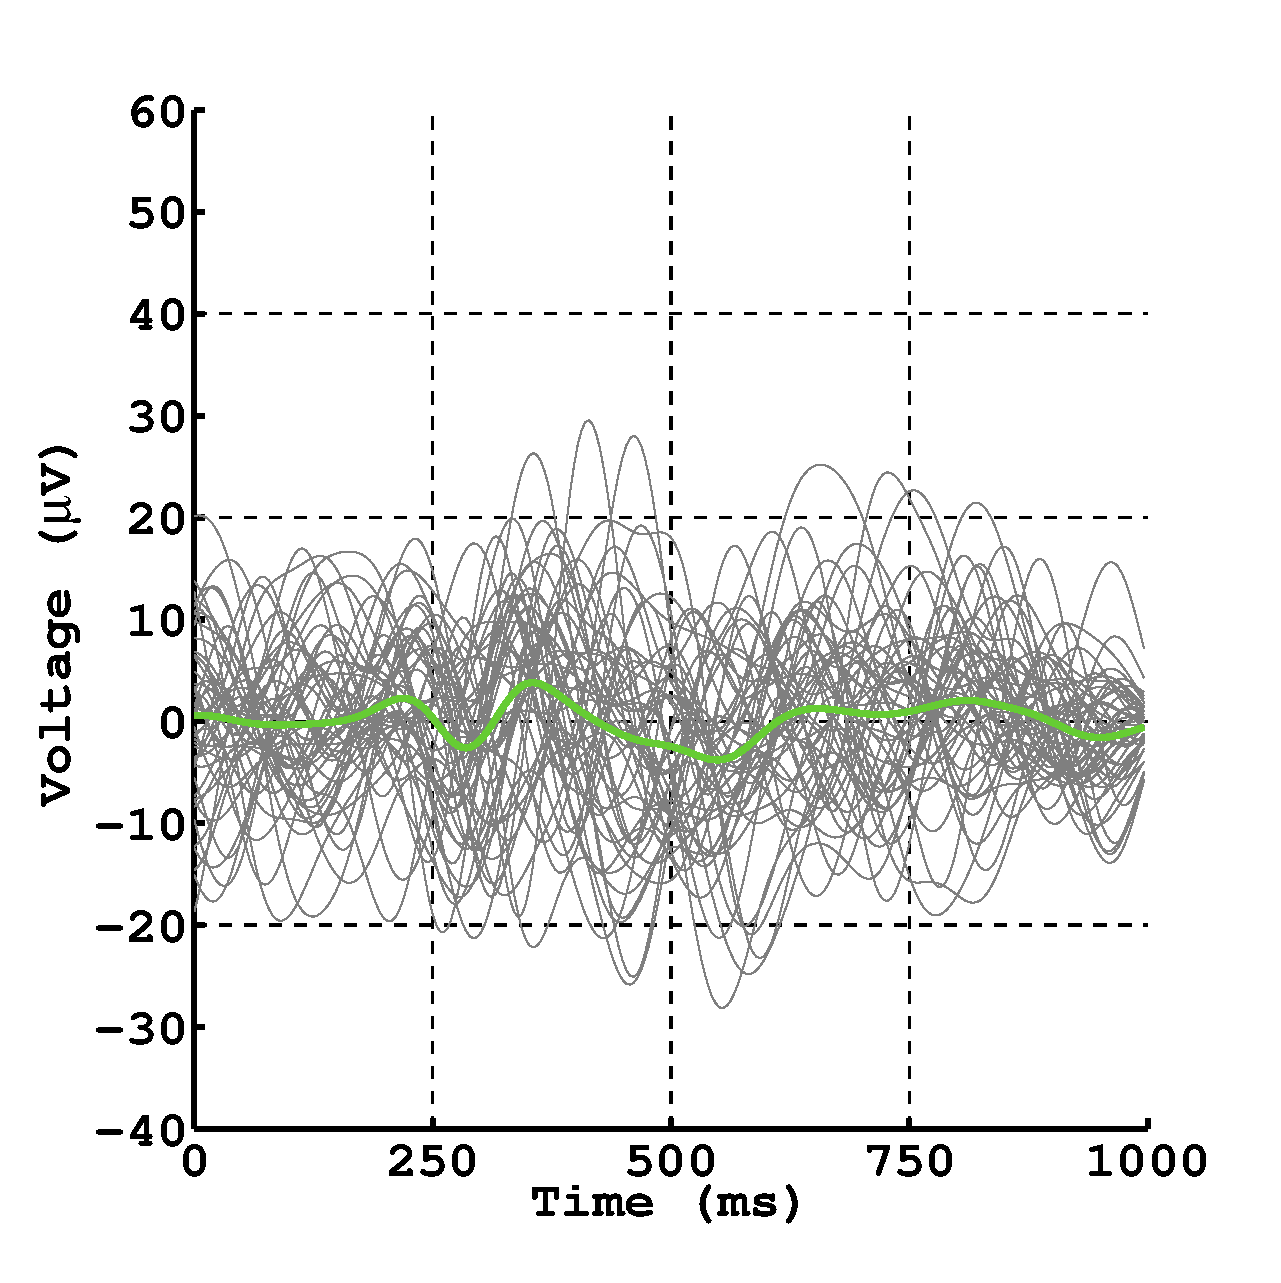
\includegraphics[width=0.49\columnwidth]{\imgpath/illustration/eeg_correct.eps}
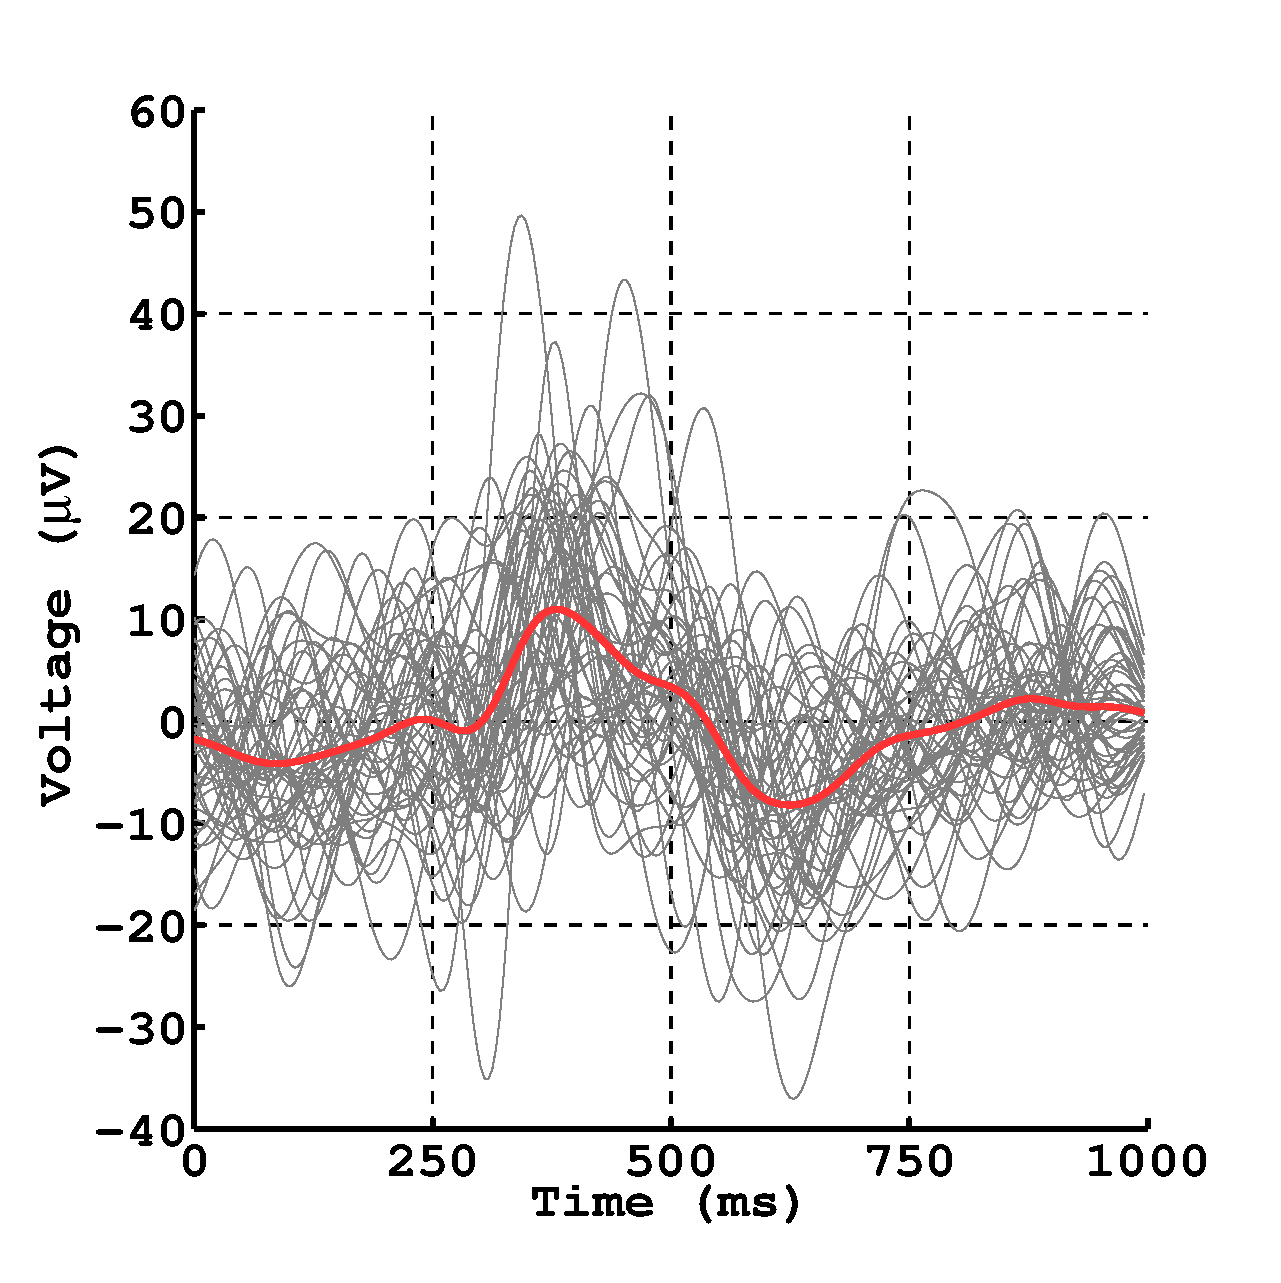
\includegraphics[width=0.49\columnwidth]{\imgpath/illustration/eeg_incorrect.eps}
\caption{Low-pass filtered EEG signals associated to ``correct'' labels (left) and to ``incorrect'' labels (right).  The signals have slightly different amplitudes, especially at around 300ms. \todo{change with one figure inkscaped}}
\label{fig:EEGsample}
\end{figure}

To build our feature vector we consider two fronto-central channels (FCz and Cz) in a time window of $[200,700]$ ms (being 0 ms the action onset of the agent) and downsampled the signal to $32$ Hz. Each element of the feature vector is the value in microvolts of the signal at the corresponding time. To compute the power information contained in our signal we simply compute the sum of the square of each feature representing our signal. This simple approximation allows to capture the slight difference in power between ``incorrect'' and ``correct'' signals (see Figure~\ref{fig:EEGpower}). However this is not enough to classify a single signal with more than 60 percent accuracy, which is almost random. But considering a group of point we can observe that the mean of power of the ``incorrect'' class is higher that the mean power of the ``correct'' class. We will exploit this property as an a priori information of which group of point should means ``correct'' or ``incorrect''.

\begin{figure}[!htbp]
\centering
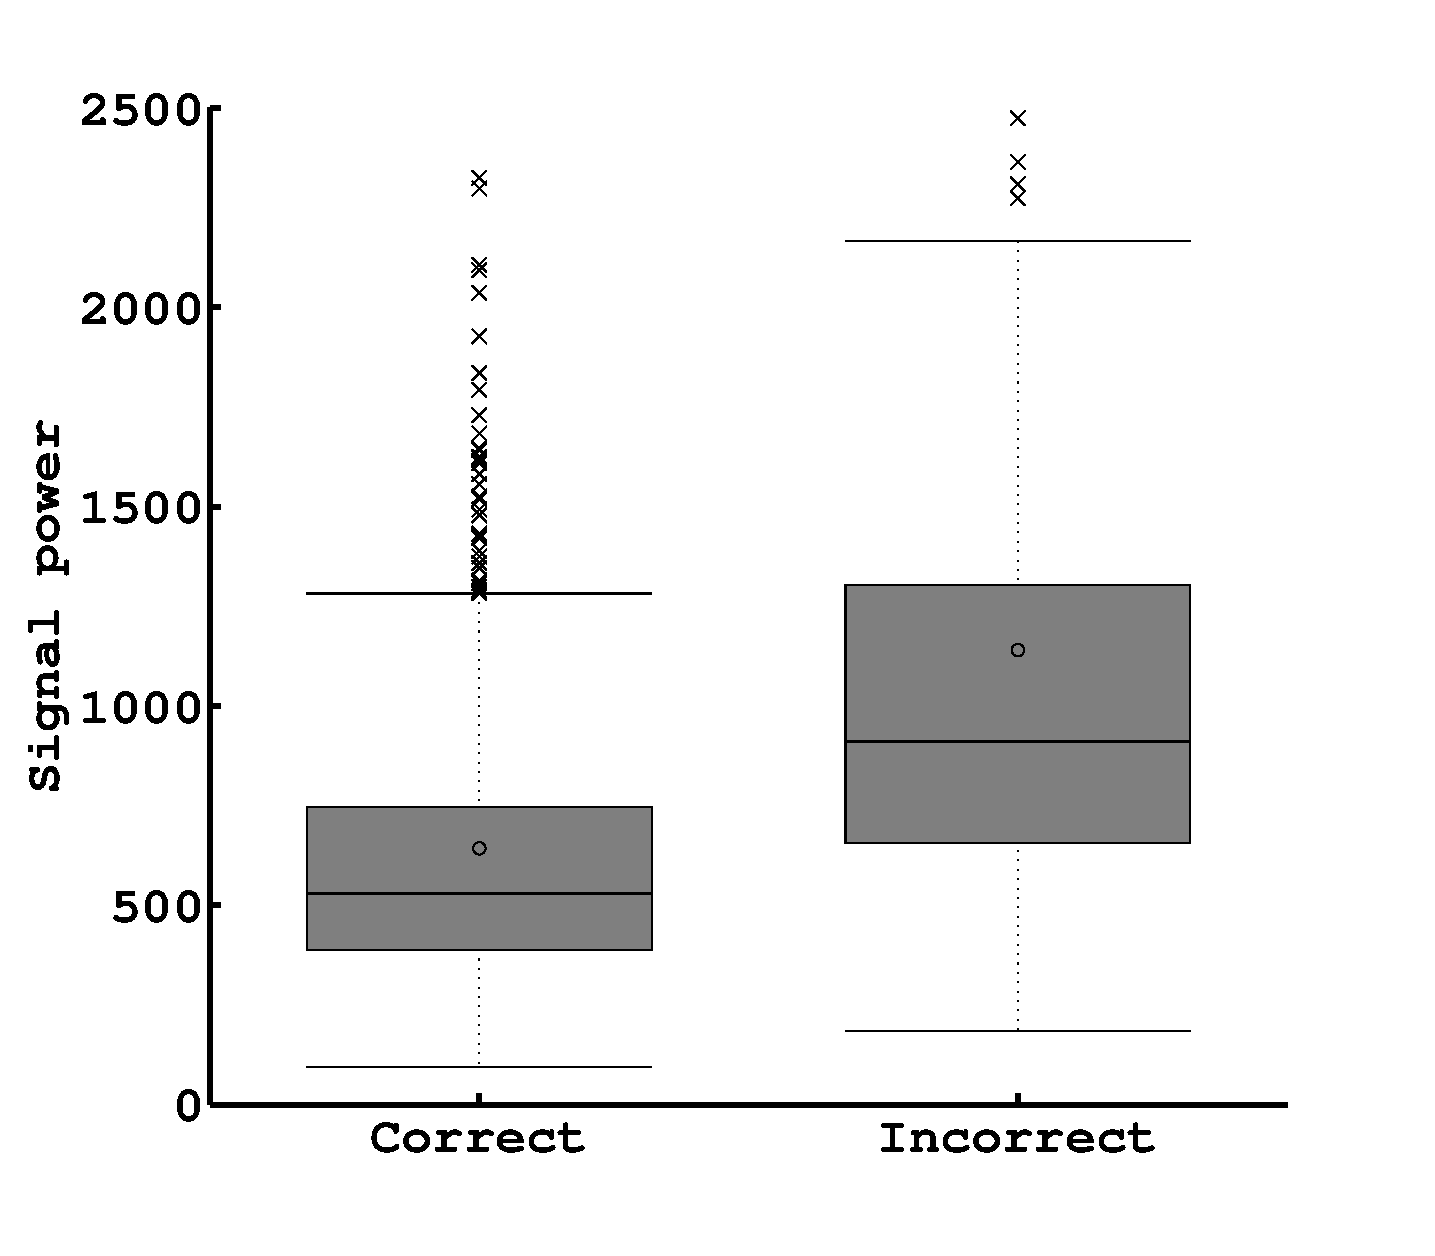
\includegraphics[width=\plotsize\columnwidth]{\imgpath/powermatching/powerdiff.eps}
\caption{Box plot of the power of ErrP signals from one of our EEG datasets. A classifier trained on this dataset reaches a classification rate of 83 percent. The mean power information from the ``incorrect'' signals is higher than for the ``correct'' ones.}
\label{fig:EEGpower}
\end{figure} 

To compute the average power information from the signals having ``correct'' labels, we simply compute the weighted mean of the signals' power, with weights the probability that each signal  being is of label ``correct''.
\begin{eqnarray}
powerCorrect(\xi_t) = \frac{\sum_{i = 1}^{M} p(l^c = ``correct"| e_i , \theta) ~~ e_i^T e_i}{\sum_{i = 1}^{M} p(l^c = ``correct"| e_i , \theta)}
\label{eq:powerCorrect}
\end{eqnarray}
with $\theta$ representing the classifier trained on the available signal-label pairs associated to the task $\xi_t$.

Similarly, for the ``incorrect'' labels, we simply compute the weighted mean of the signals' power, with weights the probability that each signal is of label ``incorrect''. 
\begin{eqnarray}
powerIncorrect(\xi_t) = \frac{\sum_{i = 1}^{M} p(l^c = ``incorrect"| e_i , \theta) ~~ e_i^T e_i}{\sum_{i = 1}^{M} p(l^c = ``incorrect"| e_i , \theta)}
\label{eq:powerIncorrect}
\end{eqnarray}
with $\theta$ representing the classifier trained on the available signal-label pairs associated to the task $\xi_t$.

For the dataset shown in Figure~\ref{fig:EEGpower}, $powerCorrect = 670$ and $powerIncorrect = 1031$. Note that this is different from the value shown by the gray circle in Figure~\ref{fig:EEGpower}. For our estimate we use the probability of each signal of being of one label as predicted by our classifier and not the probability from the training data.

Finally, we note that it is impossible to define an absolute threshold that differentiate between ``correct'' and ``incorrect'' signals (see Figure~\ref{fig:EEGpower}). 

\subsection{How to use the power information?}

As for the case of known signals described in chapter~\ref{chapter:lfui:known}, we define a specific likelihood function for the information provided by the power information, and combine it with the information from our initial algorithm. We define this likelihood as the ratio of the power associated to the ``incorrect'' class over the power of the ``correct'' class:

\begin{eqnarray}
\L_{power}(\xi_t) = \frac{powerIncorrect(\xi_t)}{powerCorrect(\xi_t)}
\label{eq:power}
\end{eqnarray}

For our previous example of Figure~\ref{fig:EEGpower}, this ratio is equal to 1.54. A ratio above 1 indicates that the labels are more likely to be correctly associated to the signals. Considering our algorithm that assigns different labels per task hypothesis and the specific case of symmetry as discussed in chapter~\ref{chapter:lfui:symmetries}. In such cases, two hypothesis have a symmetric labeling of the data, a cluster of signal considered as meaning ``correct'' for one hypothesis will be considered as being of meaning ``incorrect'' by the other hypothesis. An vice et versa. The power information breaks this symmetry. Indeed, the ``correct'' cluster should be more ``powerful'' that the ``incorrect'' cluster. In our above example, the correct hypothesis will have a power ratio of 1.54 as the label for ``incorrect'' would actually be associated to the ``incorrect'' signals. But for the symmetric case, while our non-informed algorithm could not make the difference, our new measure results in a power ratio of 0.65. Indeed, as the labels are switched, the power of class ``correct'' will be higher than the one from class ``incorrect''. Finally, considering a hypothesis whose labels are mixed, the power ratio will be around 1 because signals of low and high power will be equally distributed between ``correct'' and ``incorrect'' classes. 

We note that, disambiguating between symmetric cases is likely to improve the perceived behavior of the agent, therefore likely to improve the quality of the signals receive from the subjects. 


% However in this case our non-informed algorithm will be able to measure the change in classifier quality, which, for one of our test move from 83 percent to 61 percent classification rate.


To include the task likelihoods computed as the ratio between the power component of each classes, we simply multiply them with their respective likelihoods computed using our initial algorithm. The method is the same as described in chapter~\ref{chapter:lfui:known} when buttons of known meaning where available to the users.


% We note that measuring the ratio of power is independent from inter-subject variability in the power content of ErrP signals. 
% We note that it is impossible to define an absolute threshold that differentiate between ``correct'' and ``incorrect'' signals (see Figure~\ref{fig:EEGpower}). 


It is of crucial importance to understand the use of the power information is only possible thanks to the specific nature of the ErrP EEG signals. It would be of not use, even misleading, for the previously considered artificial 2D datasets. However other signals may have similar properties, for example, when using speech, the tone of voice may differ between ``correct'' and ``incorrect'' feedback.

Before running online EEG experiments with human subjects, we verify how the power information method behaves using our pre-recorded datasets. In next section, we compare the performance between using only the power information, only our initial algorithm, or the combination of both.

\subsection{Comparison with and without the power information}

We consider the same grid world setting presented in previous sections (e.g. section~\ref{chapter:bci:EEGsignals}) using pre-recorder EEG signals and considering a feedback frame.

\paragraph{Time to first task} Figure~\ref{fig:timefirst_powermatching} shows the number of iterations needed to reach the first target with confidence between our general method (matching), using the power information (power), or the combination of both methods (power matching). The use of the power information affects the performance for the low quality datasets (under 60 percent of accuracy). For datasets of low quality, while the time to fist target seems more advantageous when using only the power information, most of the task estimations are erroneous (see Table~\ref{tab:errorTaskRatio}), which makes the use of the power information critical for low quality data. However low quality datasets are not the main target of our algorithm. Indeed, for such data it would be better to change the representation of the brain signals or the classifier used. For datasets of higher quality (above 60 percent), the power information allows to speed up the learning compared to our initial algorithm (matching), which do not rely on known information.

\begin{figure}[!htbp]
\centering
\includegraphics[width=\plotsize\columnwidth]{\imgpath/powermatching/timefirst.eps}
\caption{Number of steps to complete the first task using EEG data. Comparison between our general method (matching), or using the information that ``incorrect'' signals are more powerful than the ``correct'' signals (power), or both methods combined (power matching). The use of the power information affects the performance for the low quality dataset (under 60 percent of accuracy). For datasets of low quality, while the time to fist target seems more advantageous when using only the power information, most of the task estimations are erroneous (see Table~\ref{tab:errorTaskRatio}), which makes the use of the power information critical for low quality data. However low quality datasets are not the main target of our algorithm. Indeed, for such data it would be better to change the representation of the brain signals or the classifier used. For datasets of higher quality (above 60 percent), the power information allows to speed up the learning compared to our initial algorithm (matching), which do not rely on known information.}
\label{fig:timefirst_powermatching}
\end{figure} 

\begin{table}
\centering
\rowcolors{2}{gray!25}{white}
\begin{tabular}{c c c c}
    Dataset Accuracies & Matching & Power & Power-Matching \\ \hline
    50-60 & 0 & 0.83 & 0.62 \\ 
    60-70 & 0 & 0.10 & 0.02 \\
    70-80 & 0 & 0.03 & 0.03 \\
    80-90 & 0 & 0.03 & 0.02 \\
    90-100 & 0 & 0 & 0 \\
\end{tabular}
\caption{Percentage of erroneous estimation of the first task using EEG data. Comparison between our general method (matching), or using the information that ``incorrect'' signals are more powerful than the ``correct'' signals (power), or both methods combined (power matching). For very low quality datasets (under 60 percent of accuracy), the power information increases the number of erroneous estimation.}
\label{tab:errorTaskRatio}
\end{table}


\paragraph{Number of tasks achieved in 500 steps}

We compare the number of tasks correctly (Figure~\ref{fig:nCorrect_powermatching}) and incorrectly (Figure~\ref{fig:nWrongEEG_powermatching}) completed in 500 steps between our general method (matching), using the power information (power), or both methods combined (power matching). The power information makes more mistakes for low quality dataset which also impacts the power matching method. However these errors occur for very low quality datasets only, which are not the main target of our algorithm. For signals above 60 percent of classification rate, the power information improves the number of tasks we can reach. 

\begin{figure}[!htbp]
\centering
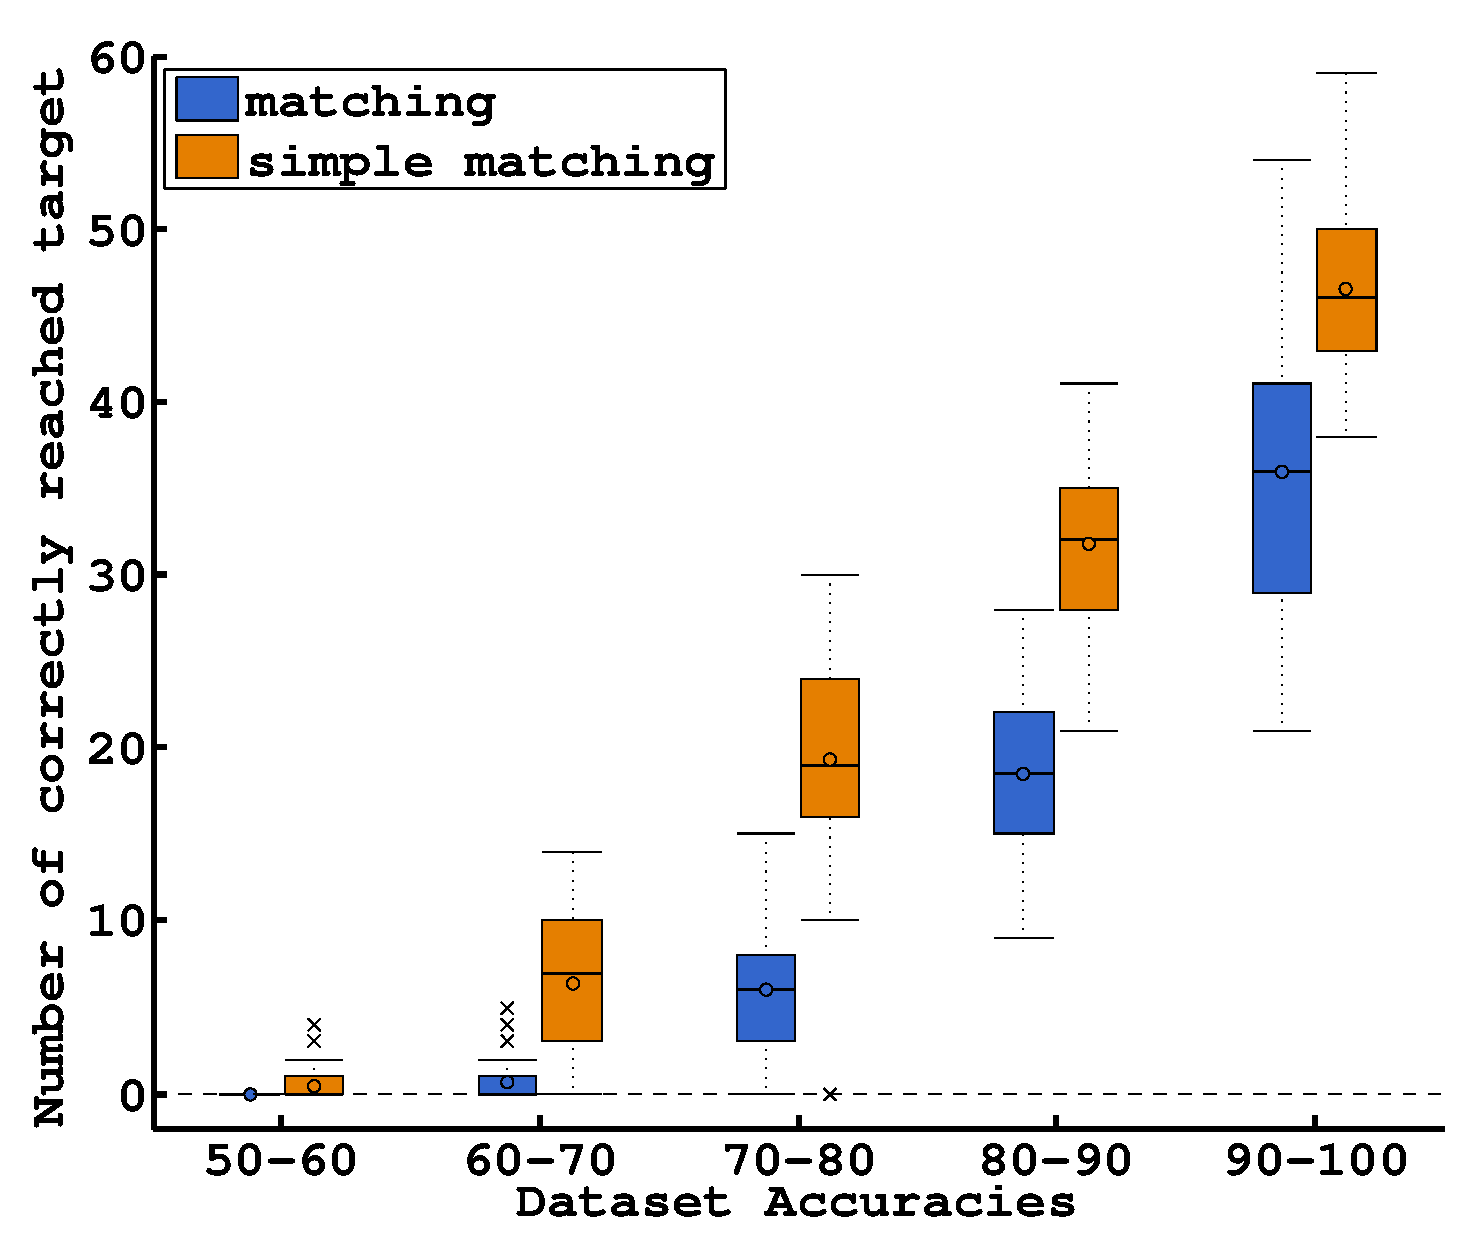
\includegraphics[width=\plotsize\columnwidth]{\imgpath/powermatching/correct.eps}
\caption{Number of tasks correctly achieved in 500 steps with EEG data. Comparison between our general method (matching), or using the information that ``incorrect'' signals are more powerful than the ``correct'' signals (power), or both method combined (power matching). The power information alone is sufficient to solve our problem but is less efficient than the other methods.}
\label{fig:nCorrect_powermatching}
\end{figure} 

\begin{figure}[!htbp]
\centering
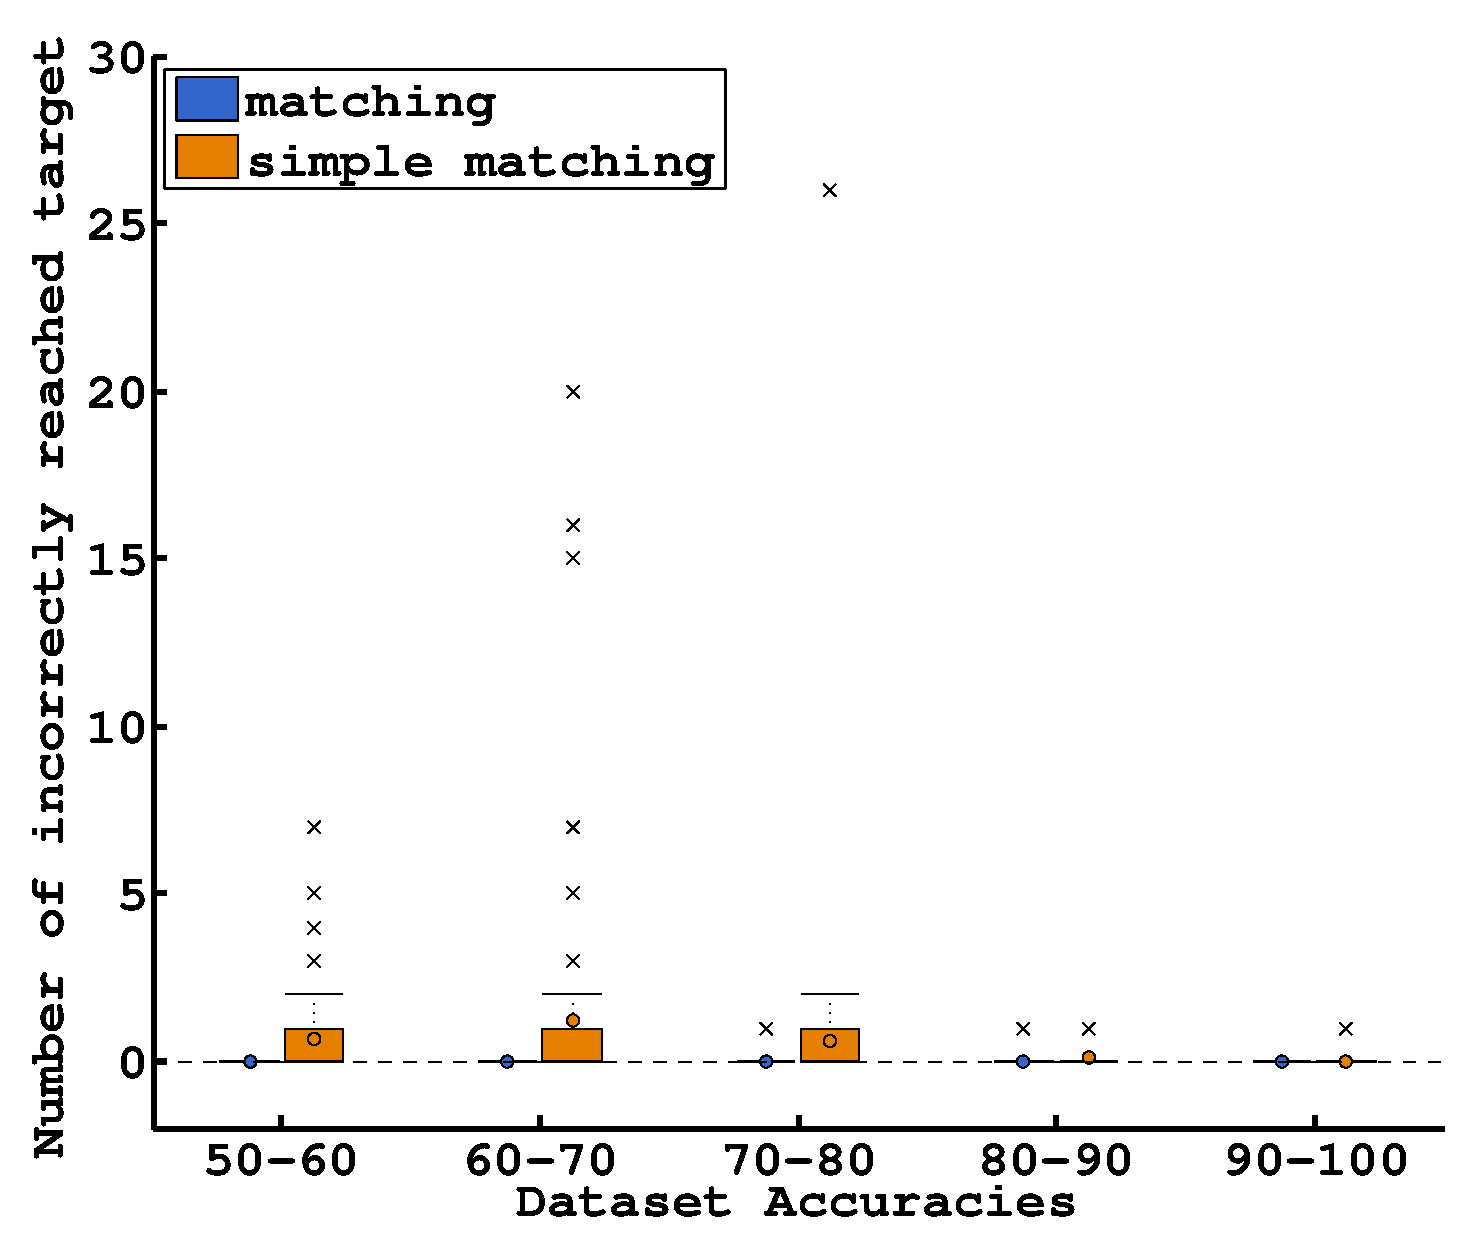
\includegraphics[width=\plotsize\columnwidth]{\imgpath/powermatching/error.eps}
\caption{Number of tasks incorrectly achieved in 500 steps with EEG data. Comparison between our general method (matching), or using the information that ``incorrect'' signals are more powerful than the ``correct'' signals (power), or both method combined (power matching). The power information makes more mistakes for low quality dataset which also impacts the power matching method. However these errors occur for very low quality datasets only, which are not the main target of our algorithm.}
\label{fig:nWrongEEG_powermatching}
\end{figure} 

The power information alone is not enough to identify a high number of task, even if the number of steps to reach the first target are similar. The difference lies in the reallocation of labels, we performed after a task is identified. As described in chapter~\ref{chapter:lfui:tasttotask}, once one task is identified with confidence, we propagate its labels to all other hypotheses. As a consequence, the number of new signals with different labels needed to pull apart two hypothesis in terms of power ratio increases. This problem arises because the power information is a global measure, which depends on averaged values over all collected observations. Our non-informed method (matching) classifies each new signal individually, which speeds up the learning process, especially when all hypothesis share a similar classifier (cf discussion of Figure~\ref{fig:sequence_evolution}).

The results presented in this section confirm that the use of the power information improves the performance and robustness of our algorithm. In addition, by disambiguating faster the task with symmetric properties, the perceived behavior of our agent should improve. We can therefore expect to receive ErrP signals of better quality during our online experiments. At the time of writing, our study was not terminated and this particular point requires a more a detailed analysis to quantify this difference if it exists.

% We can only report here our intuition from running the experiments, which is the reason of using the power information.

%%%%%%%%%%%%%%%%%%%%%%%%%%%%%%%%%%%%%%%%%%%%%%
%%%%%%%%%%%%%%%%%%%%%%%%%%%%%%%%%%%%%%%%%%%%%%
%%%%%%%%%%%%%%%%%%%%%%%%%%%%%%%%%%%%%%%%%%%%%%
%%%%%%%%%%%%%%%%%%%%%%%%%%%%%%%%%%%%%%%%%%%%%%
%%%%%%%%%%%%%%%%%%%%%%%%%%%%%%%%%%%%%%%%%%%%%%
\section{Experiments with real users}

\begin{figure}[!htbp]
\centering
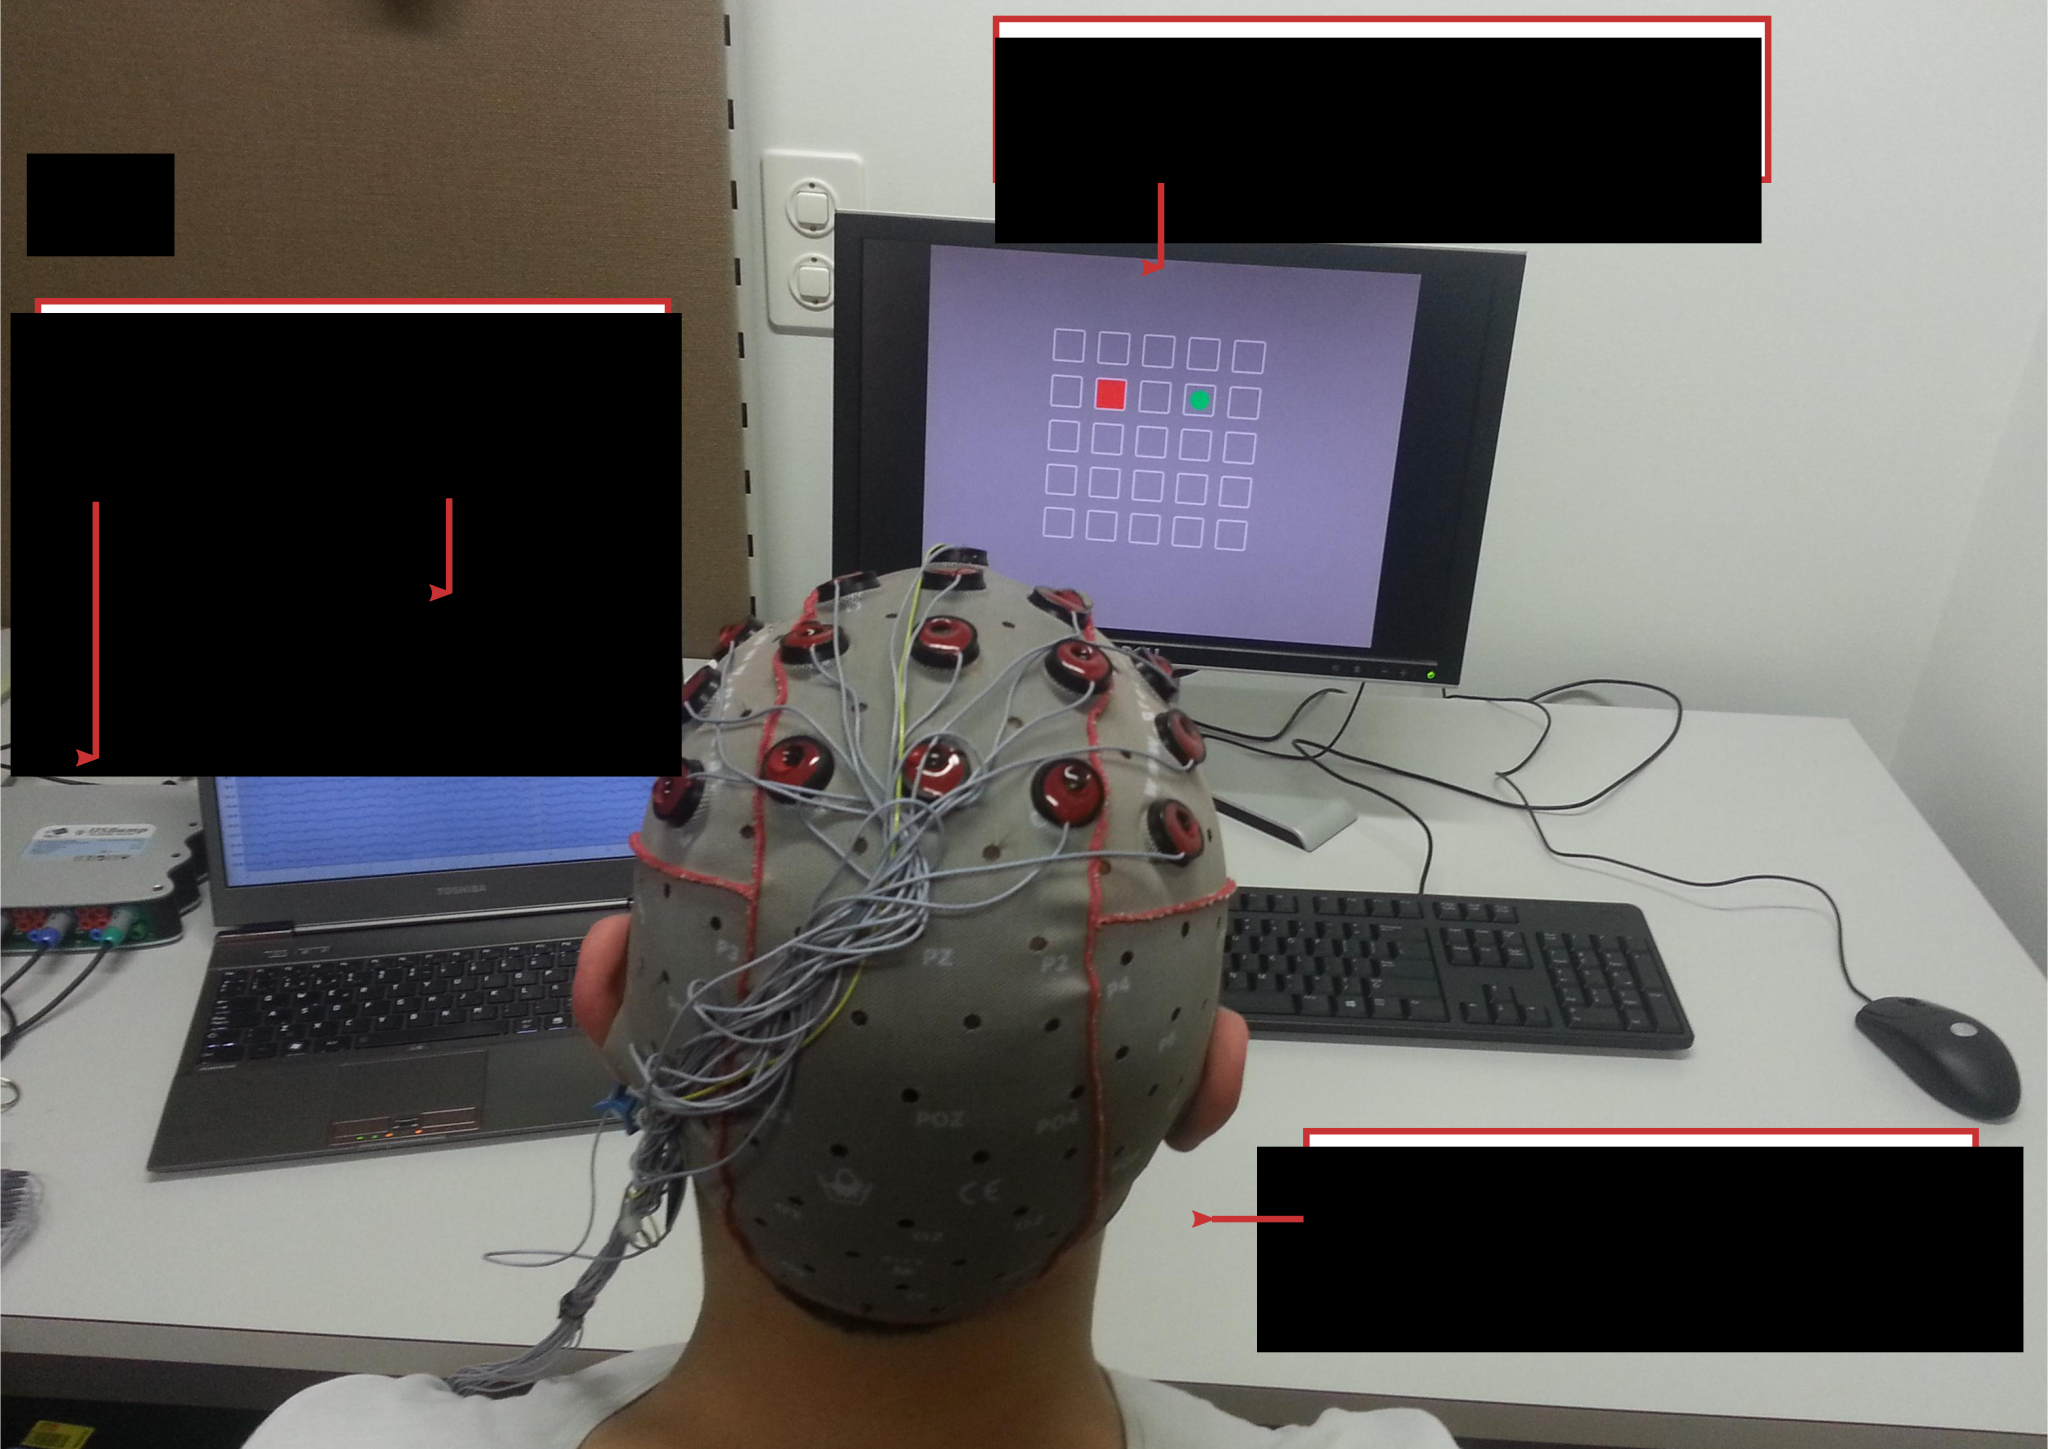
\includegraphics[width=\bcisetupsize\columnwidth]{\visualspdf/onlineXP/setup.pdf}
\caption{The BCI setup for online experiments. On the screen is displayed the grid world with the agent in green. We displayed the intended target in red, which was selected randomly. The purpose of this red square is to help the user remembering the target and our algorithm is at no point aware of the position of this red square.}
\label{fig:BCIsetup}
\end{figure}

We ran online experiments with 3 subjects. Each subject control an agent in a virtual world. The setup of our online experiment is shown in Figure~\ref{fig:BCIsetup}. Each subject was asked to mentally assess the agent's actions with respect to a given target. The system was not calibrated to decode the user EEG signals beforehand. Once the agent identified a task, and whatever the success or failure of the task identification, the user selected a new goal state randomly, the agent reseted the task likelihoods, propagates the believed labels, and teaching started again. At no point the agent has access to a measure of its performance, it could only refer to the unlabeled feedback signals from the user. There was an action every three seconds. Each experiment lasted 500 actions minimum, after 500 steps we kept running the system until a next task was reached.

As depicted in Figure~\ref{fig:correcterror_online}, our system was able to identify several tasks correctly. As for our simulated experiments, there are strong variations among subjects but we note that our system always identified the first task correctly (see Table~\ref{tab:onlineXPsummary}). Importantly, the first task was always identified in less iterations than a normal calibration procedure requires (between 300 and 600 examples depending on the user performance \cite{chavarriaga2010learning,iturrate2010single}) (see Figure~\ref{fig:timefirst_online}).


\begin{figure}[!htbp]
\centering
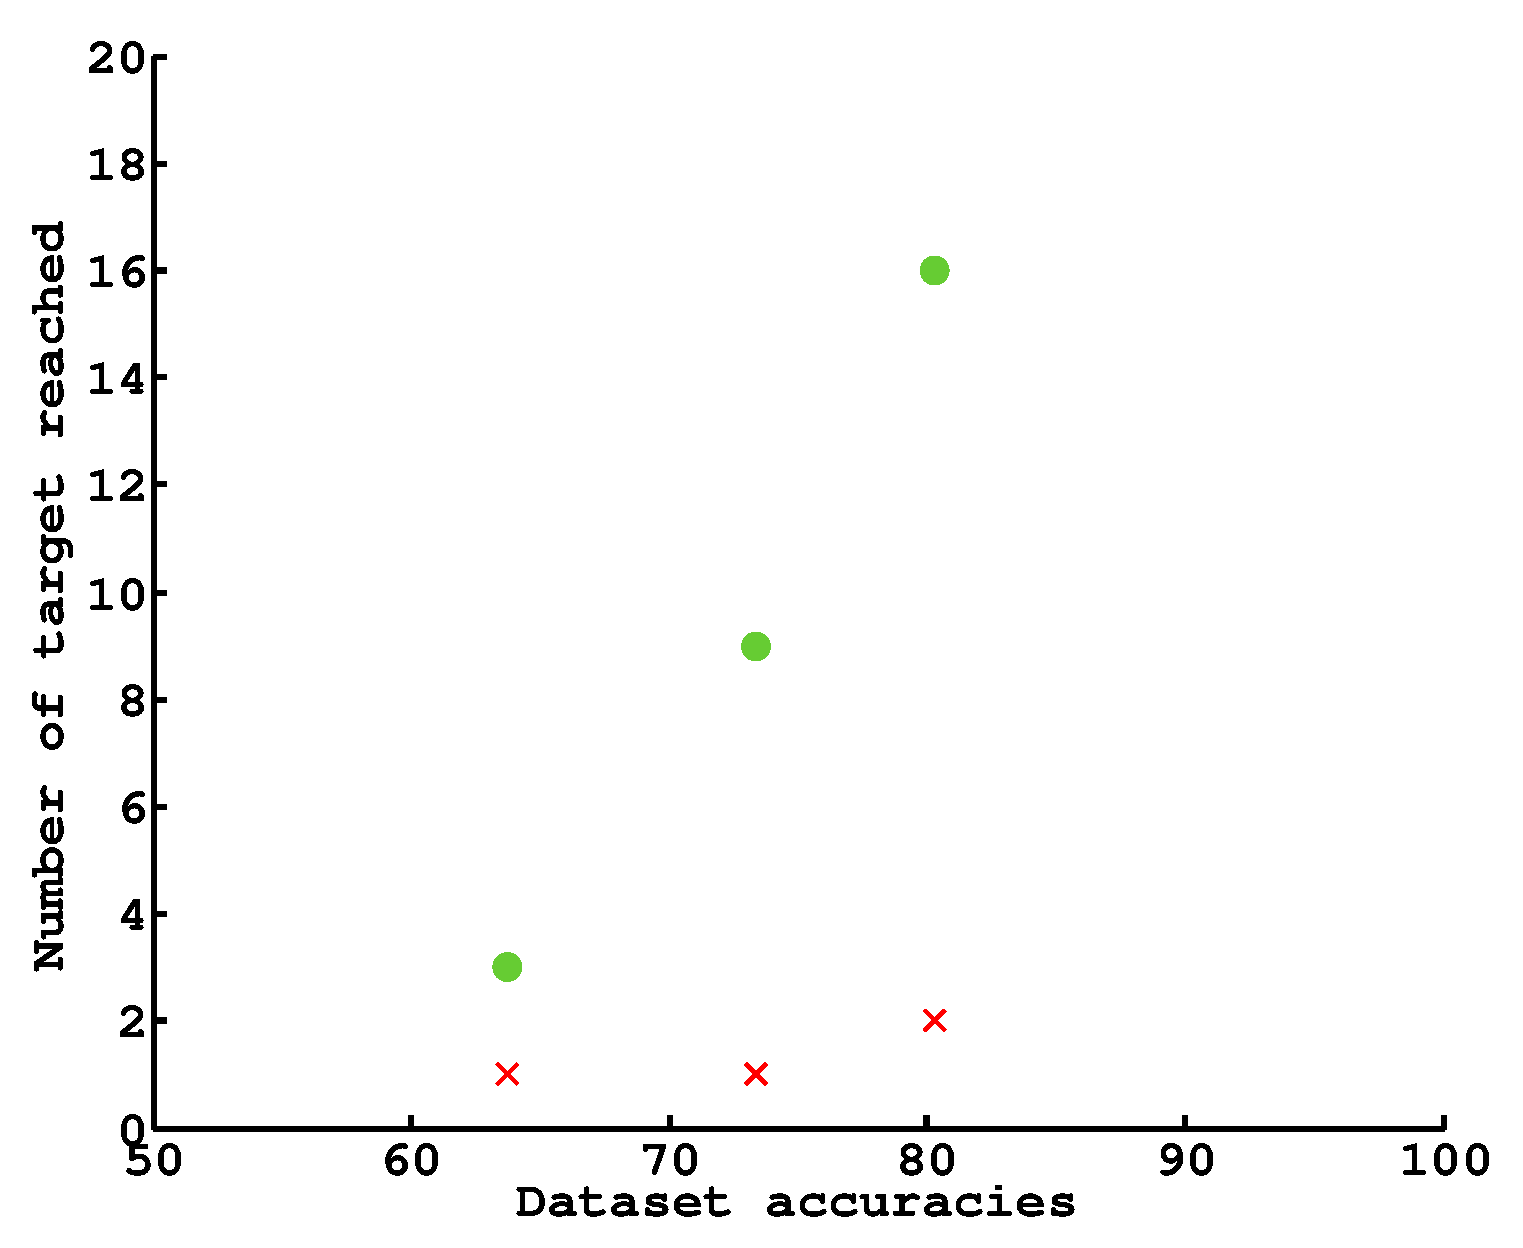
\includegraphics[width=\plotsize\columnwidth]{\imgpath/onlineXP/correct_and_error.eps}
\caption{Number of tasks correctly (green dot) and incorrectly (red crosses) achieved in 500+ steps during our online experiments with real subjects. We kept running the experiments after 500 steps until the systems identified the next task. The results are plotted against the a posteriori computed 10 fold accuracy of our classifier on each subject EEG signals. The performance of the system is correlated with the quality of the EEG signals. These results matches well with the results from simulated experiments.}
\label{fig:correcterror_online}
\end{figure} 


\begin{figure}[!htbp]
\centering
\includegraphics[width=\plotsize\columnwidth]{\imgpath/onlineXP/timefirst.eps}
\caption{Number of steps to complete the first task for all subjects in our online experiments. The results are plotted against the a posteriori computed 10 fold accuracy of our classifier on each subject EEG signals. The relation between data quality and the time to first task is in line with our simulated results shown in Figure~\ref{fig:timefirst_powermatching}. Note that the first target was evaluated correctly for every subject.}
\label{fig:timefirst_online}
\end{figure} 


\begin{table}
\centering
\rowcolors{2}{gray!25}{white}
\begin{tabular}{c c c c c c}
    Subject & Class. rate & Steps to first task & First correct & N. correct & N. error\\ \hline
    S1 & 80 & 101 & Yes & 16 & 2\\ 
    S2 & 73 & 131 & Yes & 9 & 1\\
    S3 & 64 & 265 & Yes & 3 & 1\\
\end{tabular}
\caption{Results from our online experiments. For each subject, we provide the a posteriori computed classification rate of classifier on subject's brain signals (Class. rate), the number of steps needed to identify the first task, and whether or not the task identified was the correct one. Finally, we give the number of task that were correctly and incorrectly identified in 500 steps.} 
\label{tab:onlineXPsummary}
\end{table}

% \begin{figure}[!htbp]
% \centering
% 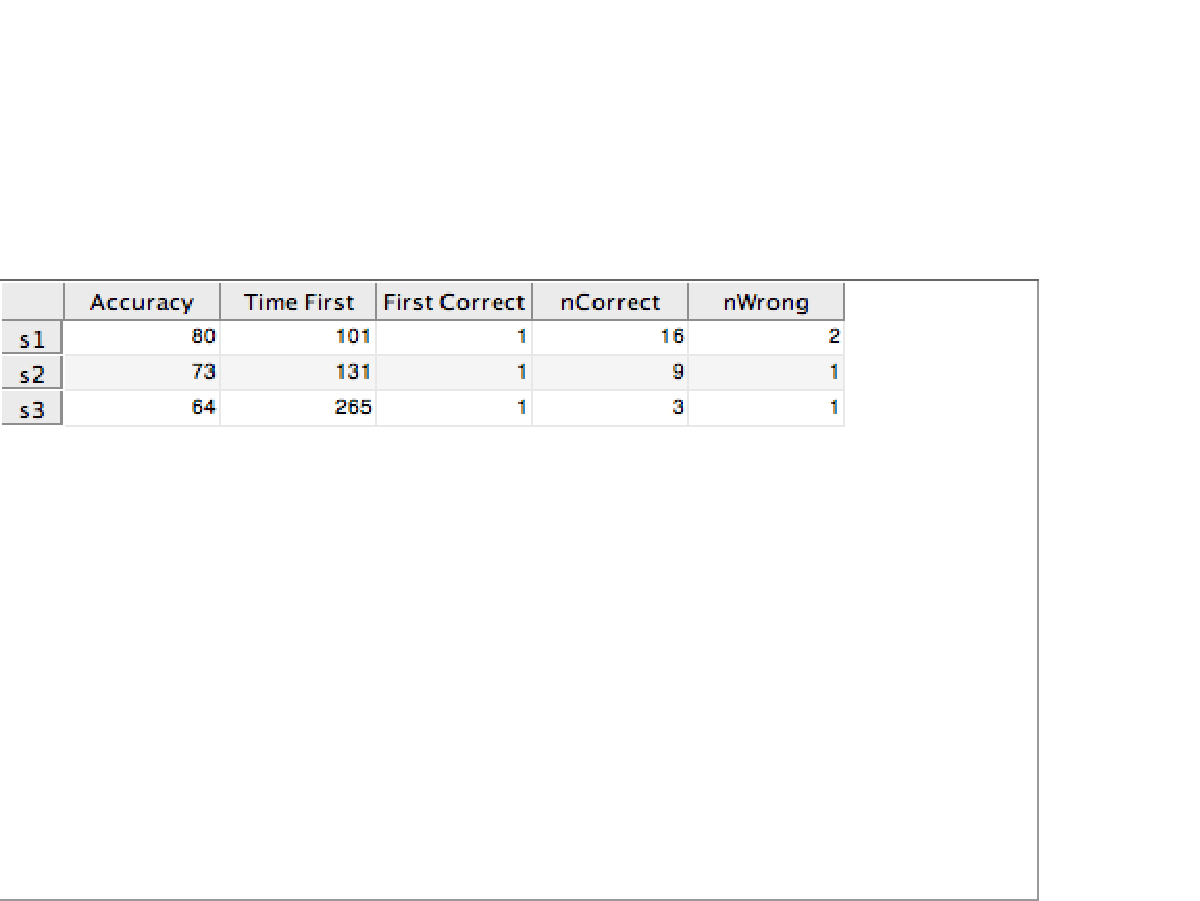
\includegraphics[width=\columnwidth]{\imgpath/onlineXP/table.png}
% \caption{\todo{change with a latex table}}
% \label{fig:correcterror_online}
% \end{figure} 

\transition

Results presented in this chapter with real EEG signals allow us to envision that the algorithm presented in this thesis could have practical applications in the real word. By removing the need of an expert to collect and calibrate the system, the use of brain computer interfaces may become more practical allowing their users to go out of the labs.

While this work offers a good solution to start interacting with machines without defining in advance the particular signals that will be used by the users, we have only demonstrated its performances on relatively simple scenarios. Especially, we considered discrete states and actions, synchronous protocol, and a finite set of task hypothesis. While these constraints have no impact on most BCI scenarios, they are a more limiting factor for robotics experiments. In next chapter, we address some of these limitations in simple experiments, which may provide ideas for the future developments of this work.

% accuracy = 0.83
% powerCorrect = 670
% powerWrong = 1031
% ratio = 1.54
% ratio symmetric = 0.65
% accuracy shuffle = 0.61
% ratio shuffle = 1.00


% \begin{figure}[!htbp]
% \centering
% 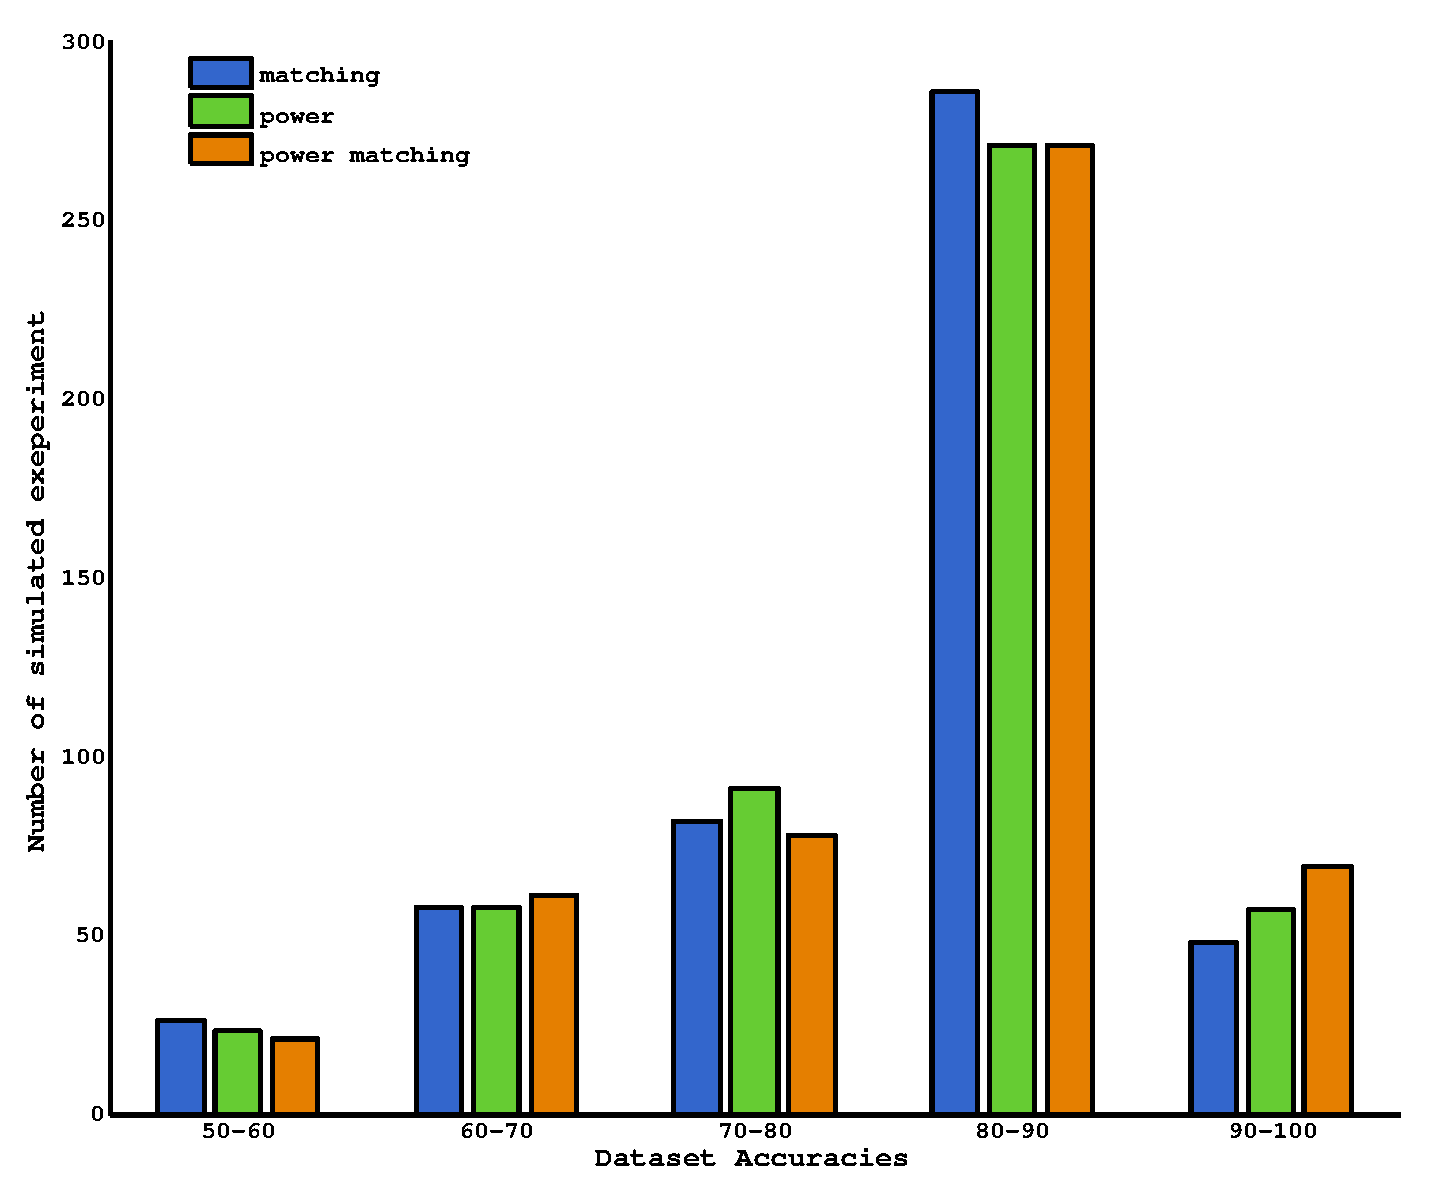
\includegraphics[width=\plotsize\columnwidth]{\imgpath/powermatching/nSim.eps}
% \caption{\todo{use a table instead of this figure}}
% \label{fig:nSim_powermatching}
% \end{figure} 


% nSim =

%   Columns 1 through 3

%     26    58    82
%     23    58    91
%     21    61    78

%   Columns 4 through 5

%    286    48
%    271    57
%    271    69

% ratioFirstWrong =

%   Columns 1 through 2

%          0         0
%     0.8261    0.1034
%     0.6190    0.0164

%   Columns 3 through 4

%          0         0
%     0.0330    0.0332
%     0.0256    0.0185

%   Column 5

%          0
%          0
%          0


% \begin{figure}[!htbp]
% \centering
% 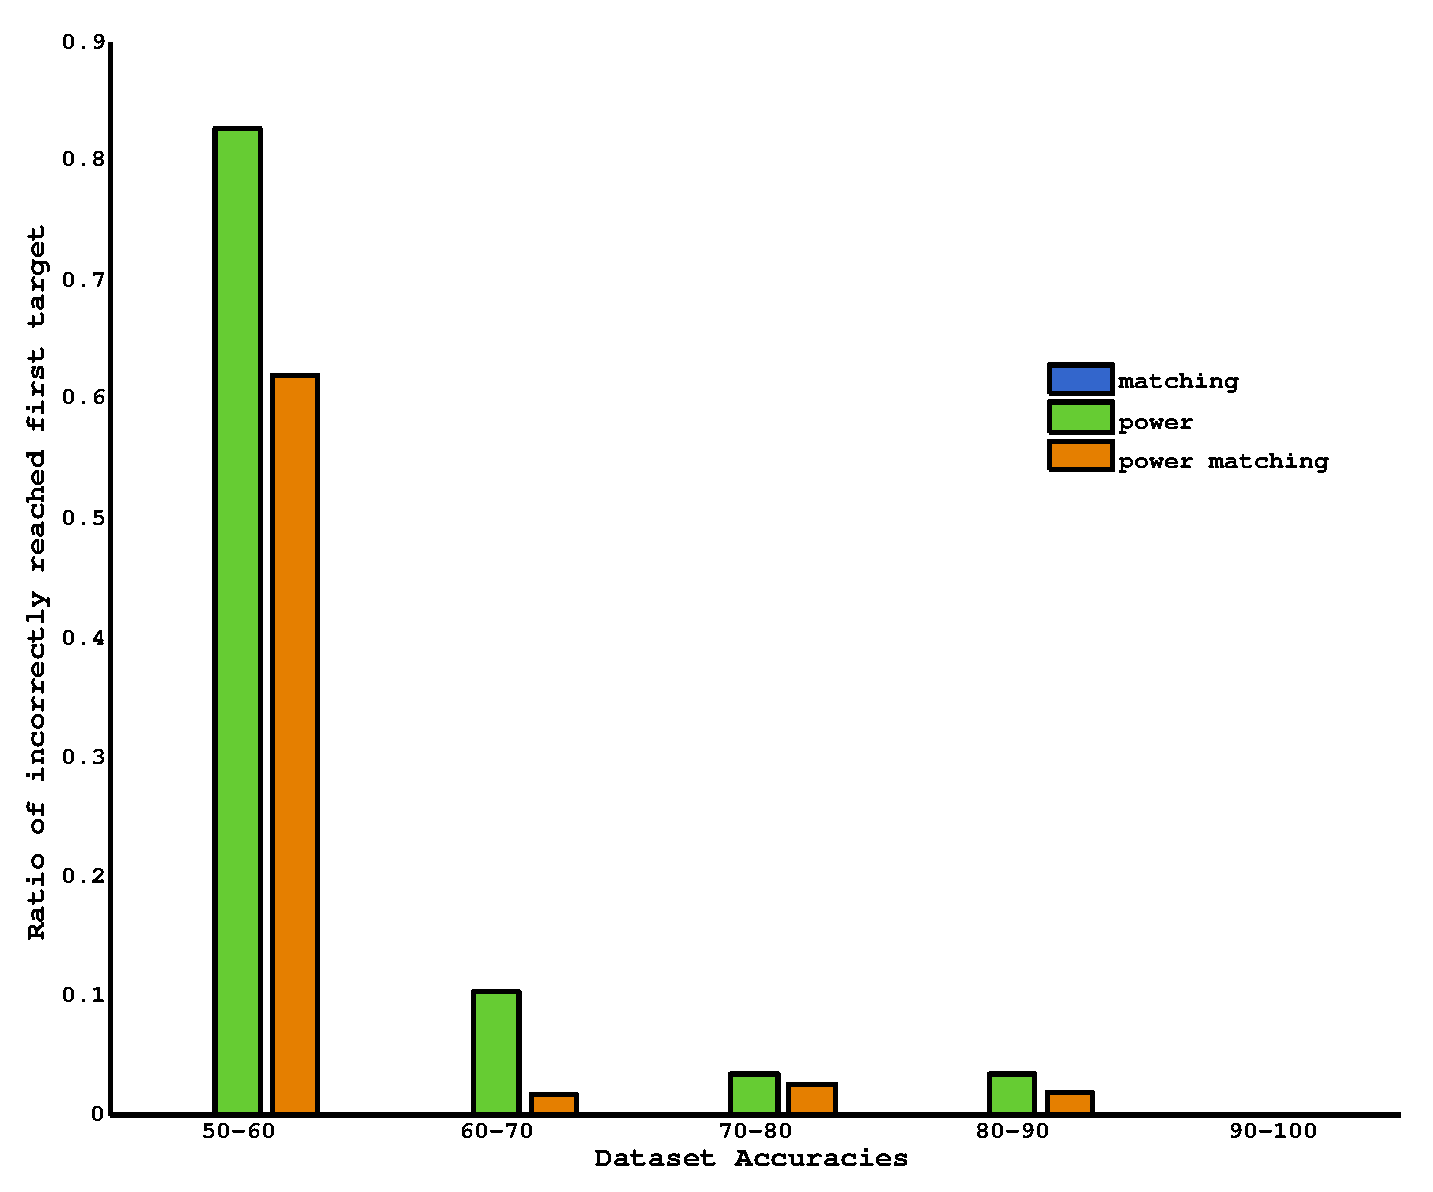
\includegraphics[width=\plotsize\columnwidth]{\imgpath/powermatching/errorfirst.eps}
% \caption{Percentage of time the first task estimated was erroneous using EEG data. Comparison between our general method (matching), or using the information that ``incorrect'' signals are more powerful than the ``correct'' (power), or both method combined (power matching). For low quality datasets, the power information increases the number of erroneous estimation. However those errors occurs for very low quality datasets, which are not the main target of our algorithm.}
% \label{fig:errorfirst_powermatching}
% \end{figure} 
